\section{Non signal testing of the regular and variational Autoencoder}


\subsection*{Autoencoder}
Both the large and small autoencoder produced results, and are shown below. The small autoencoder results will always be first for each of the tests. 
\subsubsection*{Channel removing}

\begin{figure}[h!]
    \centering
    \begin{subfigure}{.8\textwidth}
        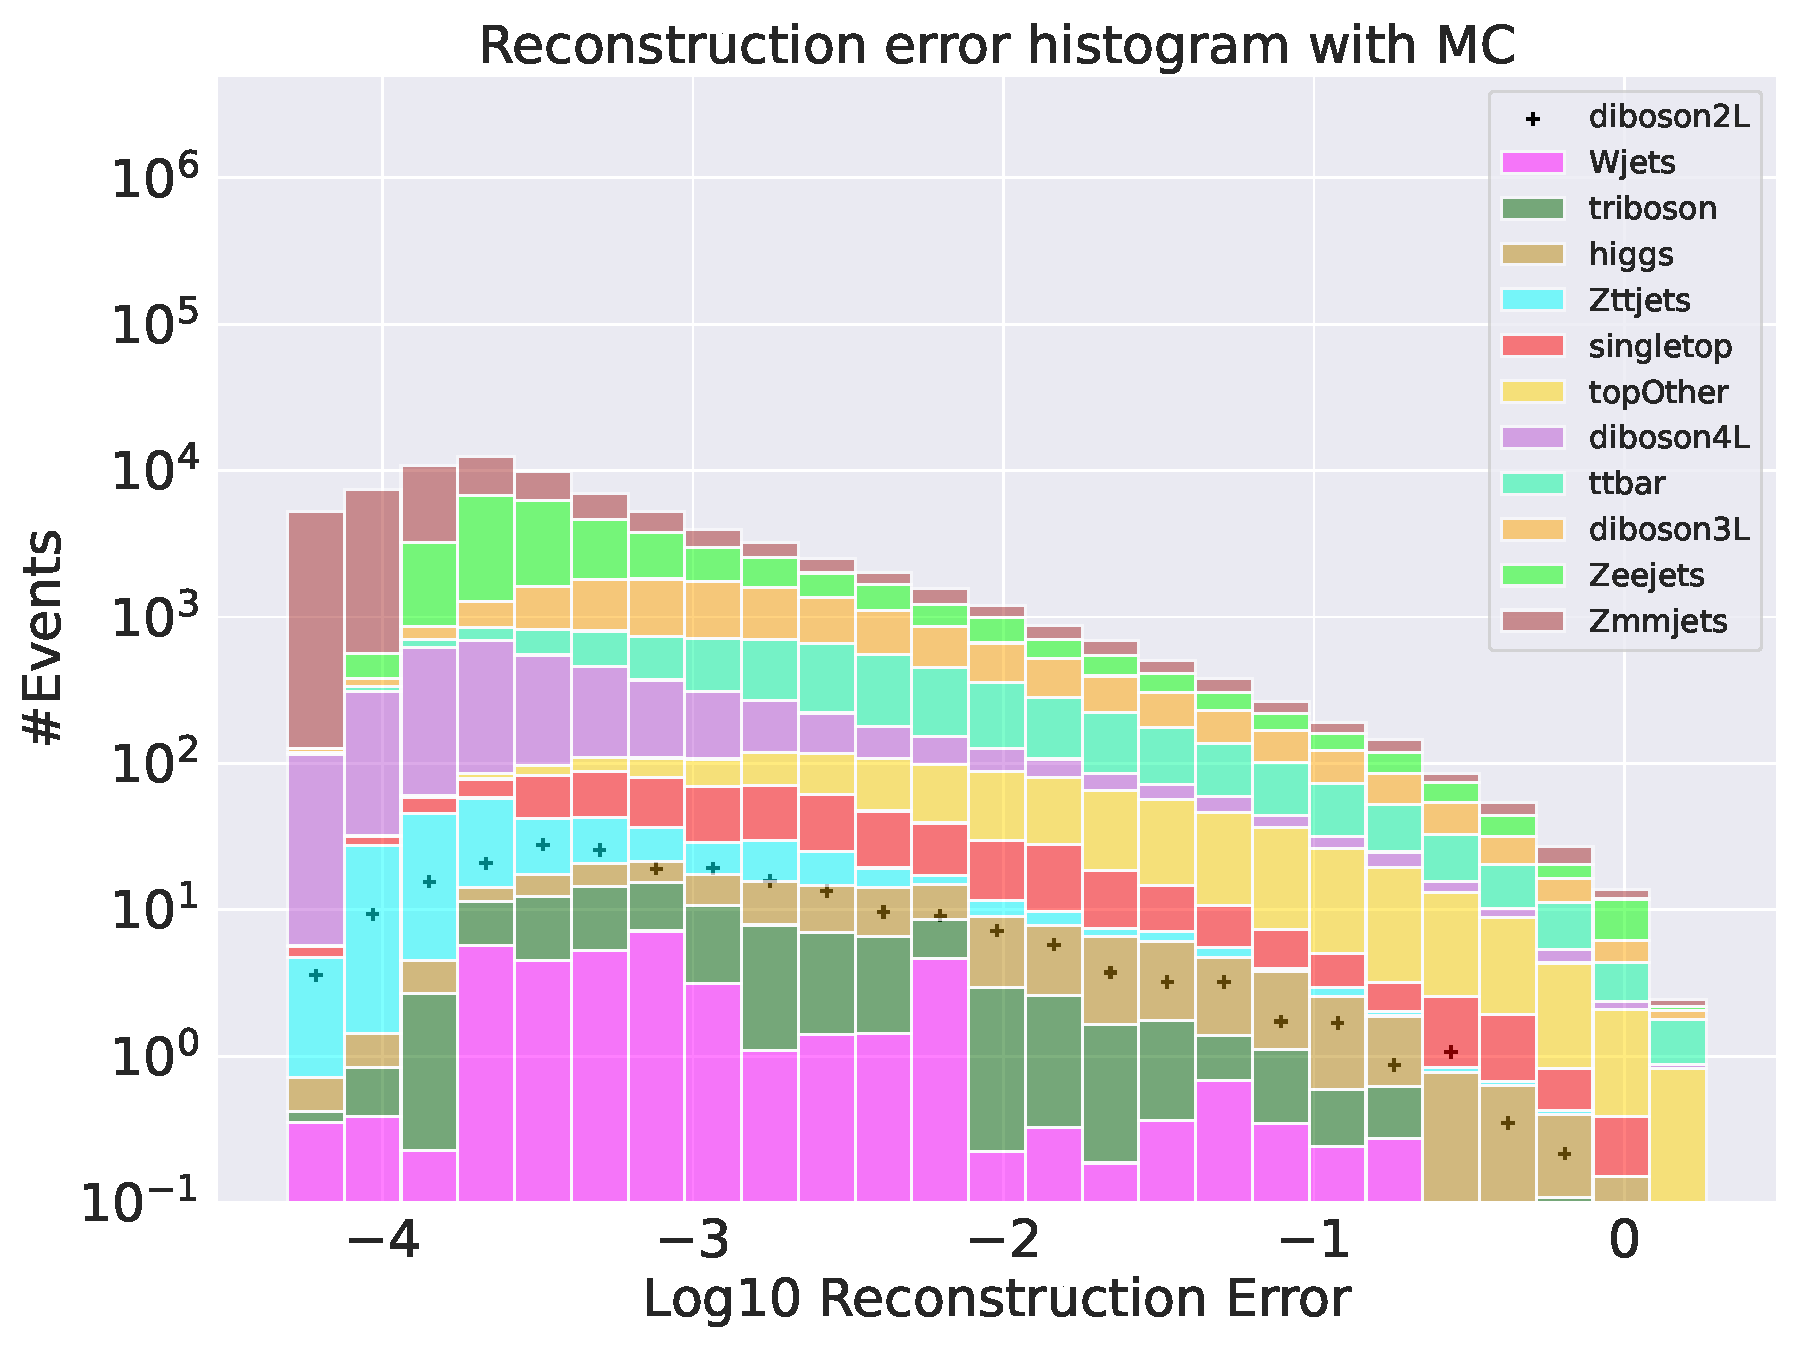
\includegraphics[width=\textwidth]{Figures/AE_testing/small/b_data_recon_big_rm3_feats_sig_diboson2L.pdf}
        \caption{Reconstruction error on validation SM MC from the Autoencoder. Here the diboson2l channel has been removed from training and 
        is used as signal. No significant difference in distributions are found.}
        \label{fig:ae_small_diboson2l}
    \end{subfigure}
    \hfill
    \begin{subfigure}{.8\textwidth}
        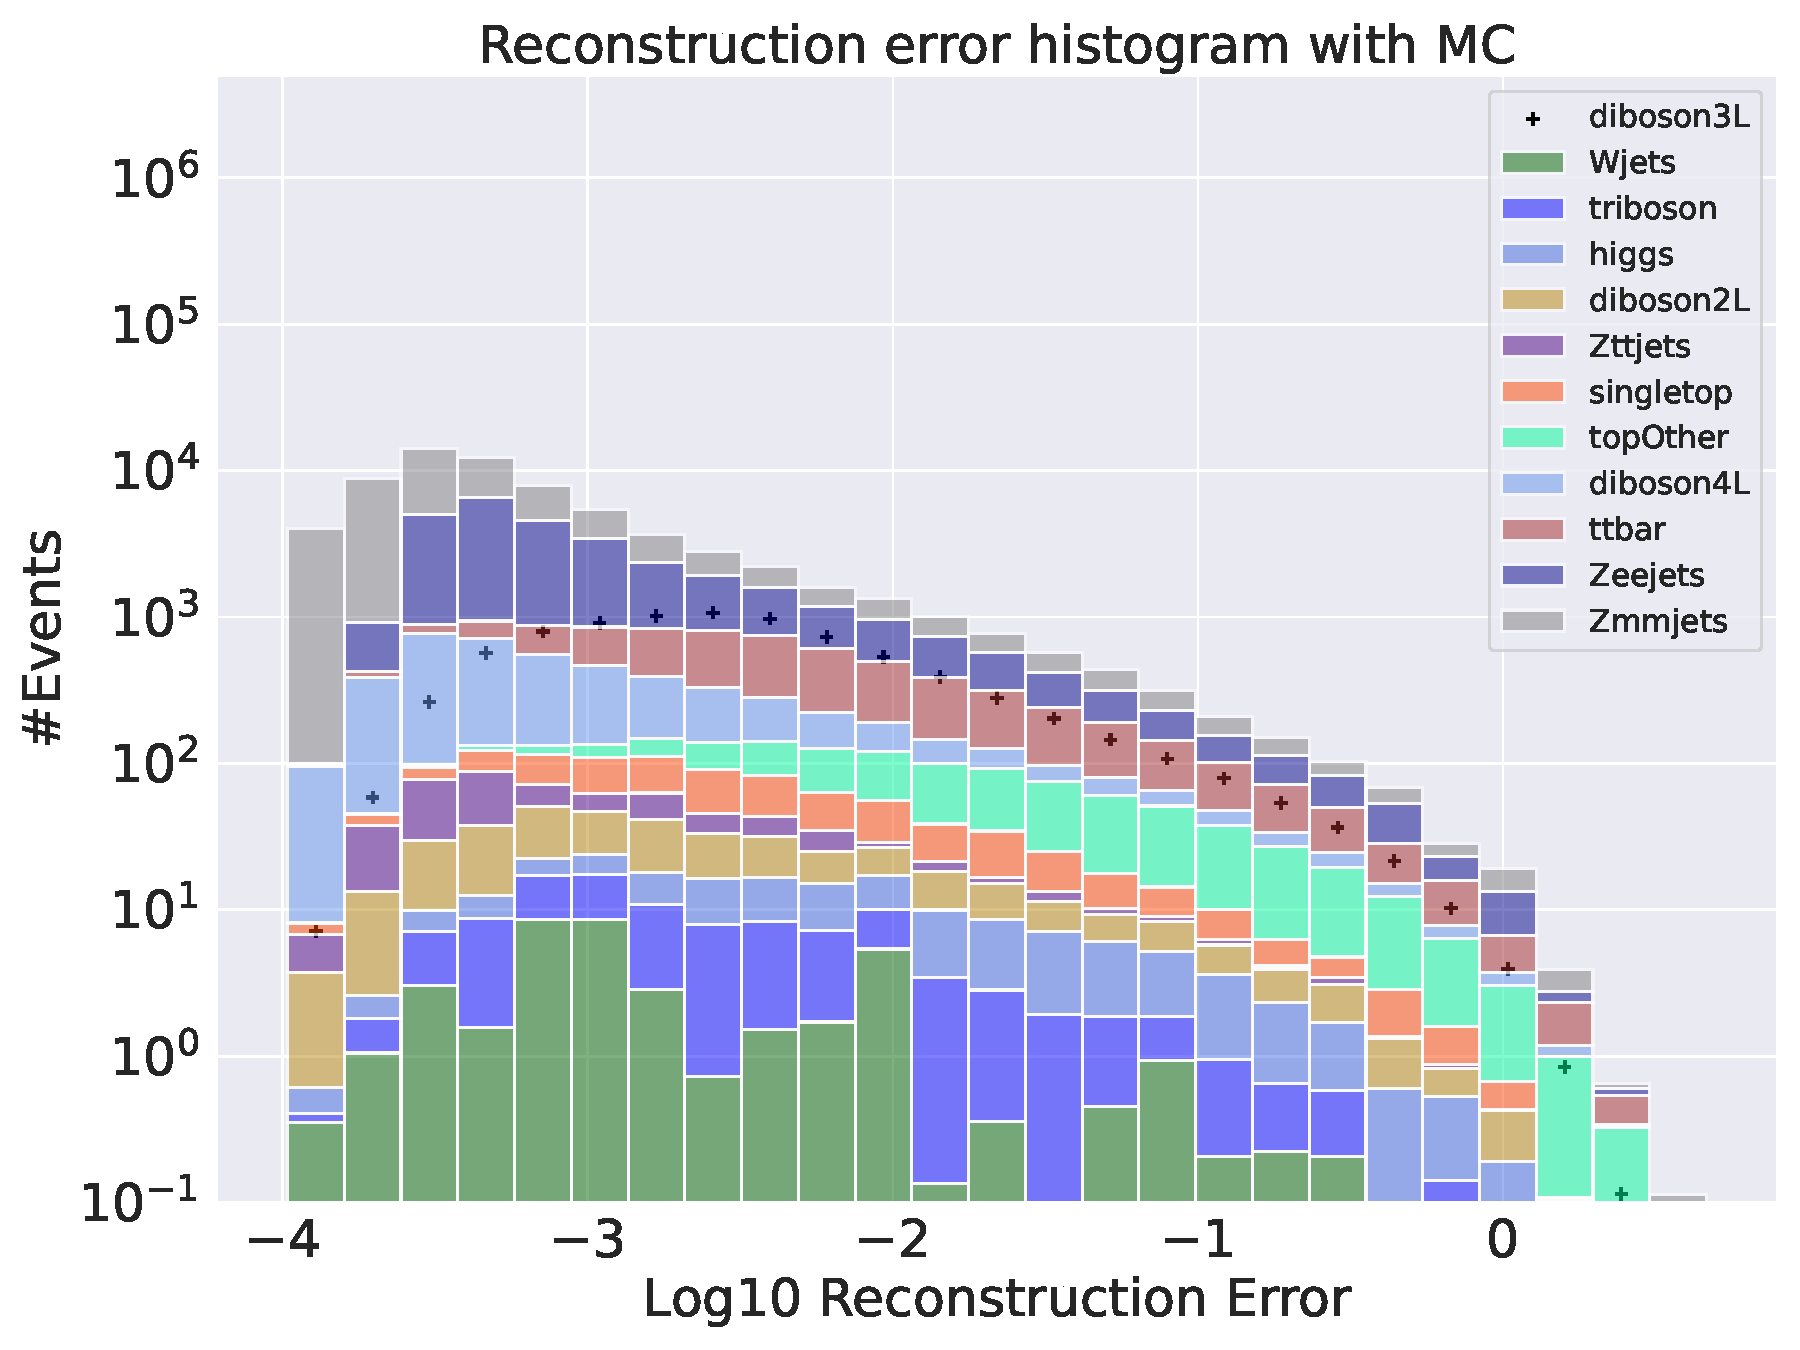
\includegraphics[width=\textwidth]{Figures/AE_testing/small/b_data_recon_big_rm3_feats_sig_diboson3L.pdf}
        \caption{Reconstruction error on validation SM MC from the Autoencoder. Here the diboson3l channel has been removed from training and 
        is used as signal. No significant difference in distributions are found.}
        \label{fig:ae_small_diboson3l}
    \end{subfigure}
    \hfill        
    \caption{ }
    \label{fig:ae_small_channel1}
\end{figure}

\begin{figure}[h!]
    \centering
    \begin{subfigure}{.8\textwidth}
        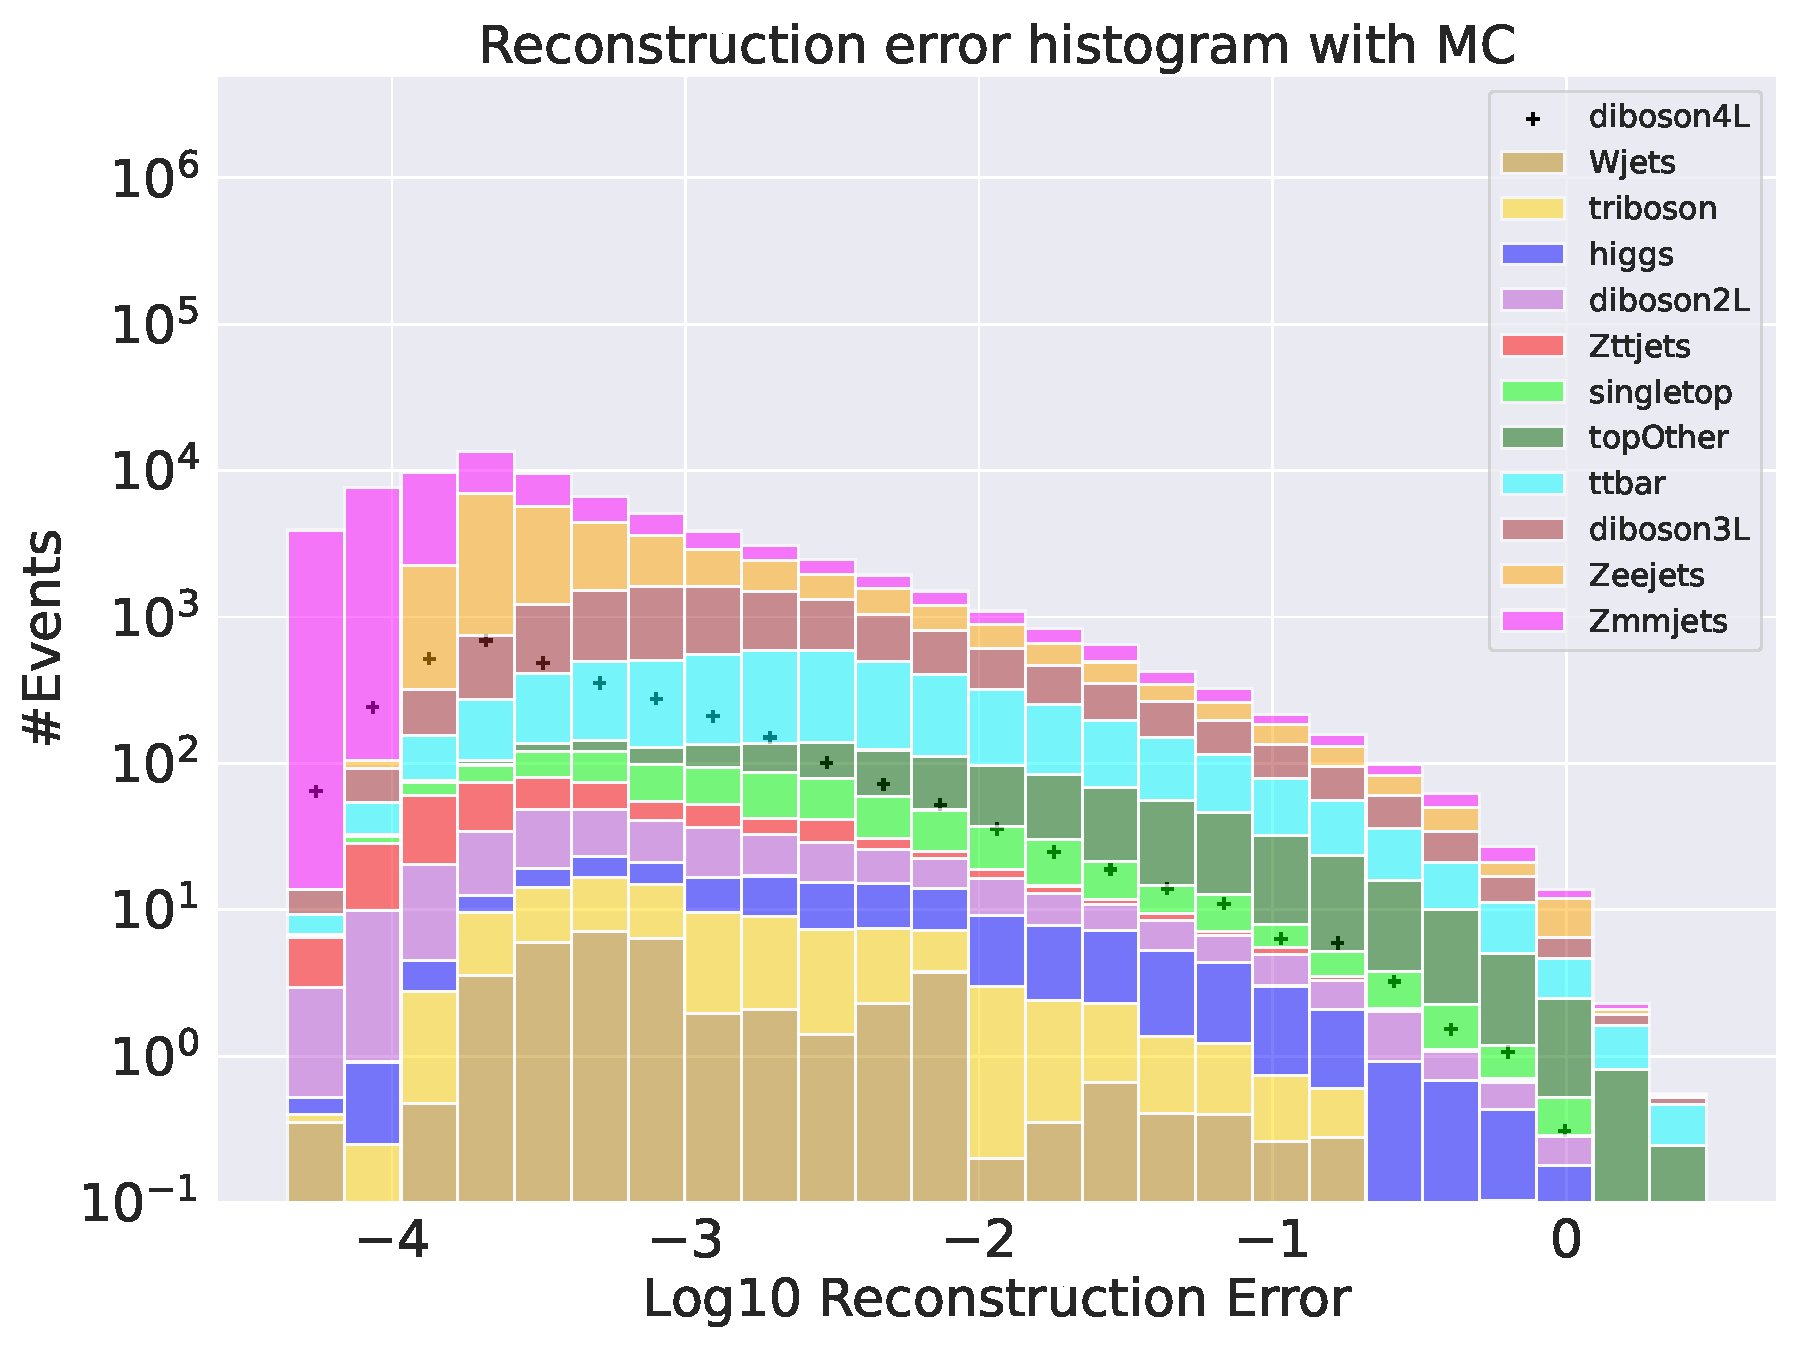
\includegraphics[width=\textwidth]{Figures/AE_testing/small/b_data_recon_big_rm3_feats_sig_diboson4L.pdf}
        \caption{Reconstruction error on validation SM MC from the Autoencoder. Here the diboson4l channel has been removed from training and 
        is used as signal. No significant difference in distributions are found. }
        \label{fig:ae_small_diboson4l}
    \end{subfigure}
    \hfill
    \begin{subfigure}{.8\textwidth}
        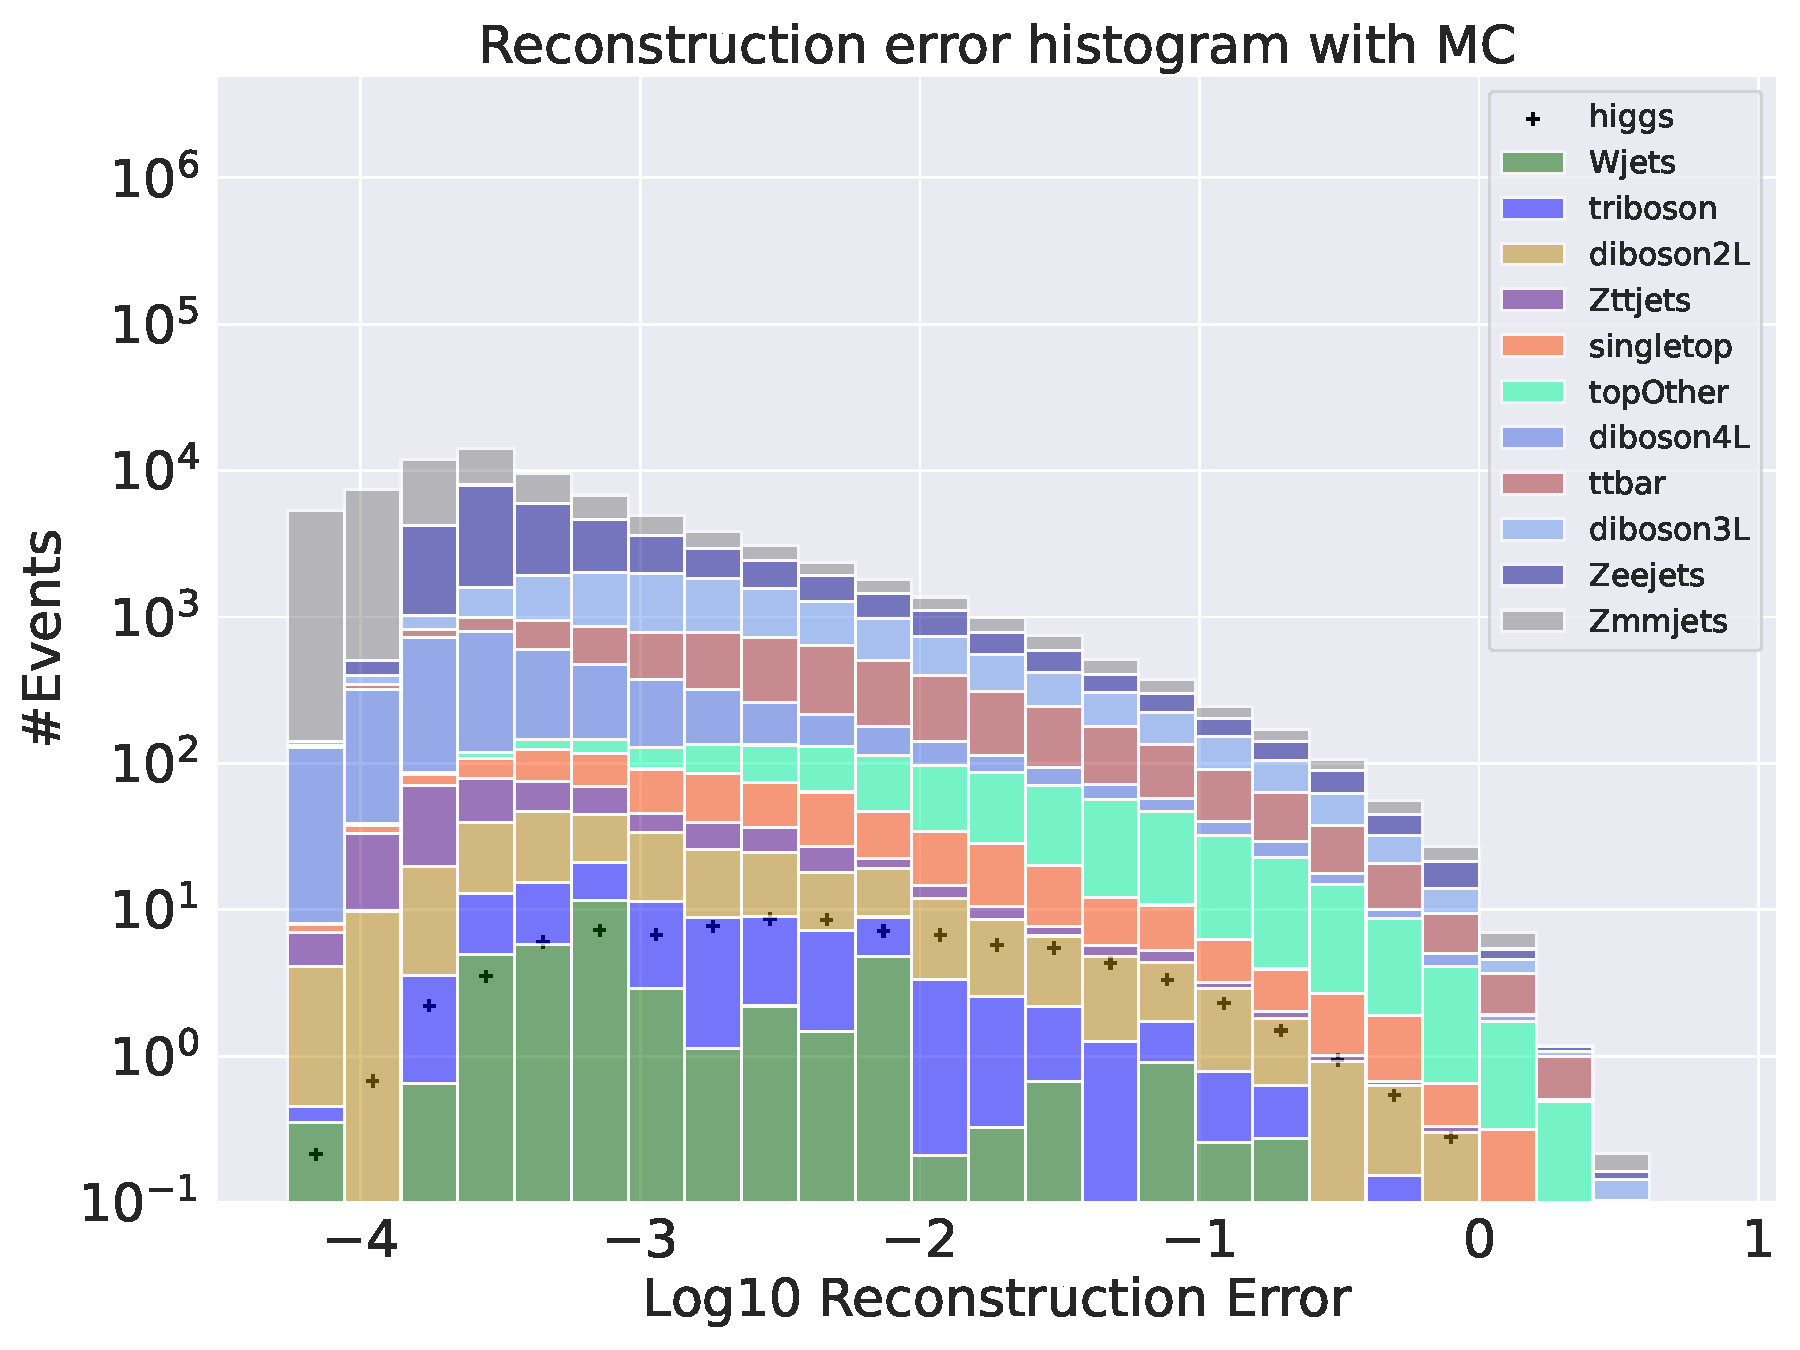
\includegraphics[width=\textwidth]{Figures/AE_testing/small/b_data_recon_big_rm3_feats_sig_higgs.pdf}
        \caption{Reconstruction error on validation SM MC from the Autoencoder. Here the higgs channel has been removed from training and 
        is used as signal. No significant difference in distributions are found.}
        \label{fig:ae_small_higgs}
    \end{subfigure}
    \hfill        
    \caption{ }
    \label{fig:ae_small_channel2}
\end{figure}

\begin{figure}[h!]
    \centering
    \begin{subfigure}{.8\textwidth}
        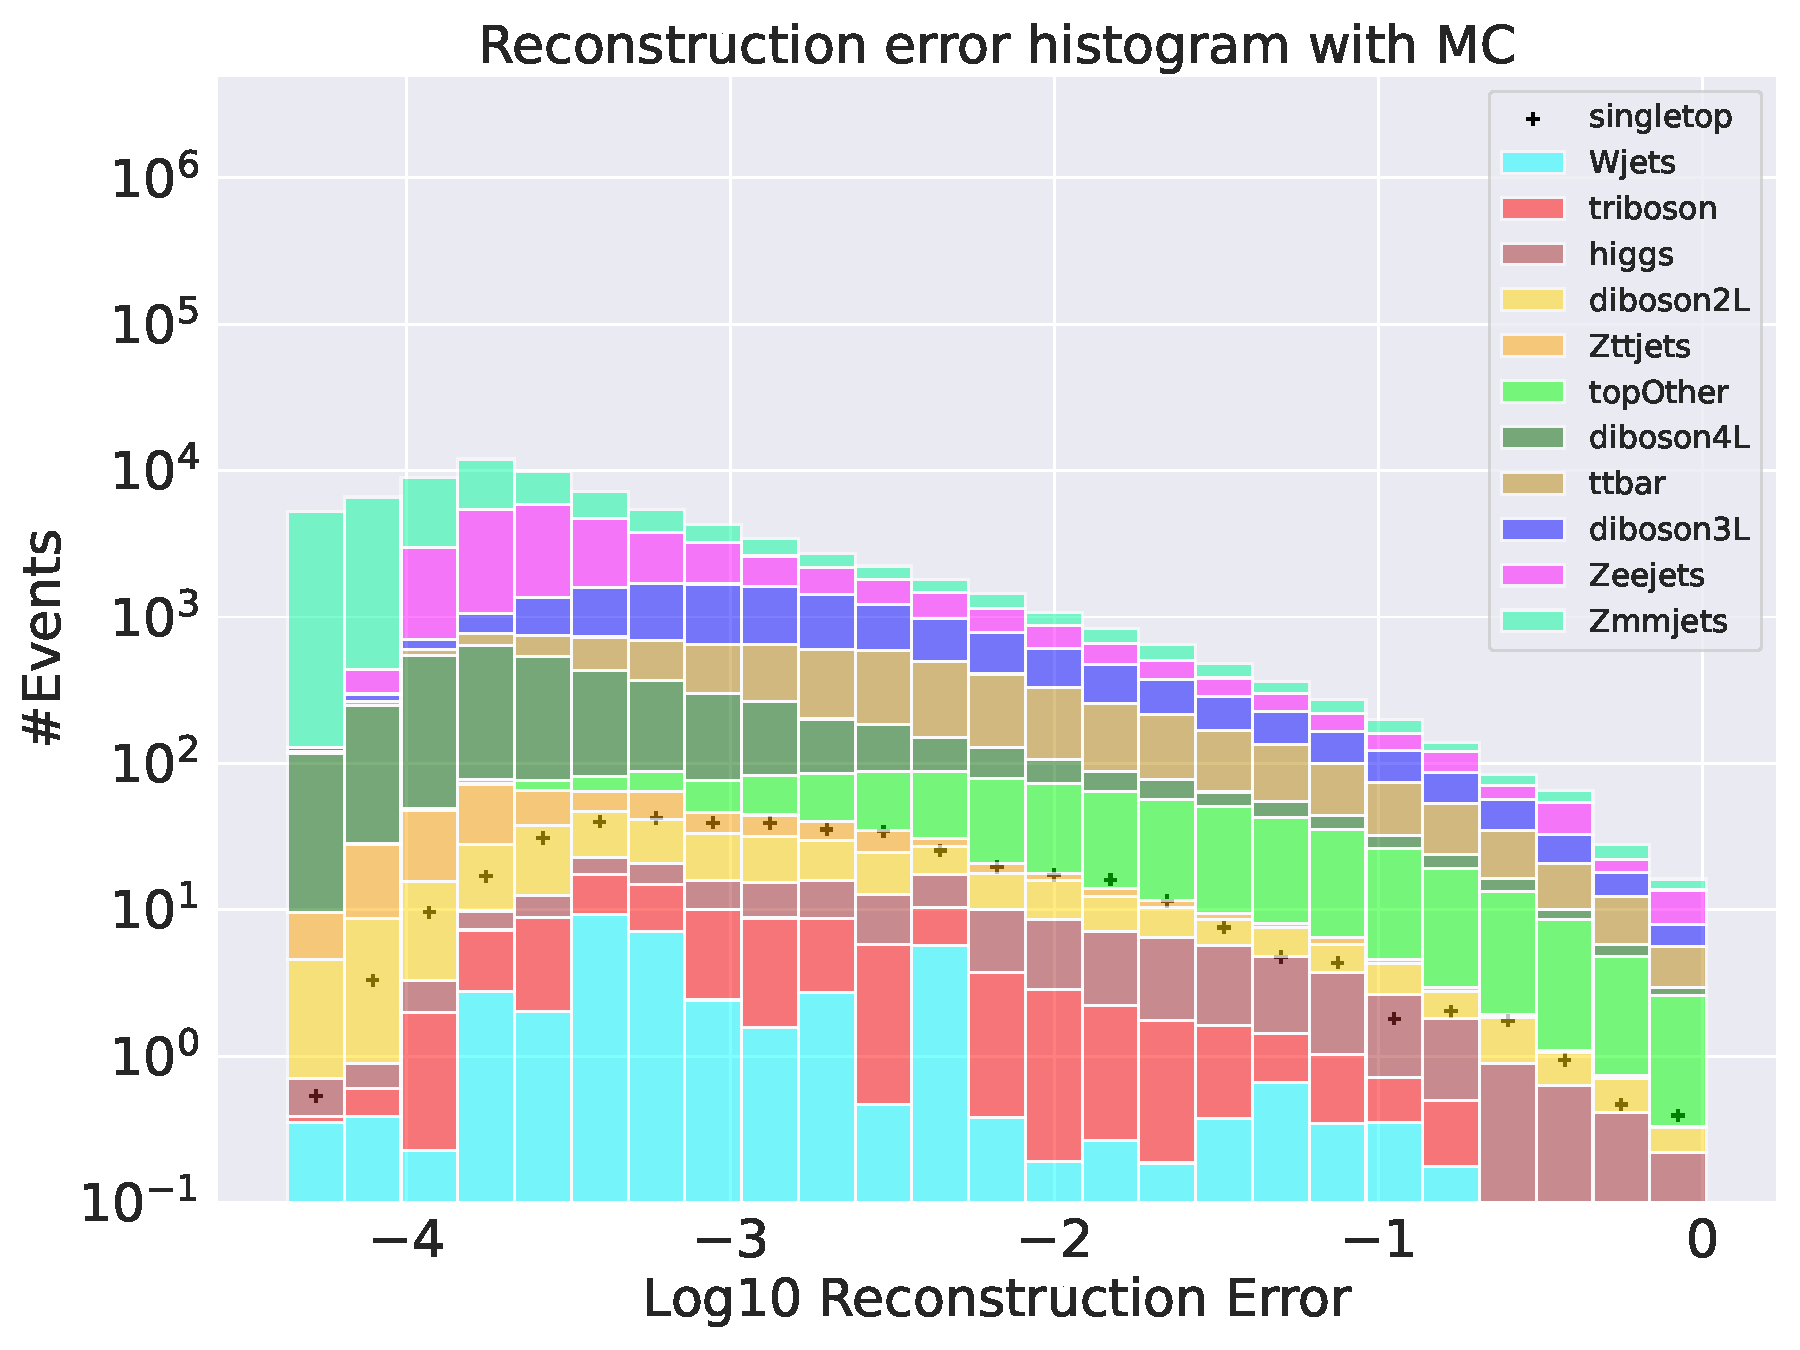
\includegraphics[width=\textwidth]{Figures/AE_testing/small/b_data_recon_big_rm3_feats_sig_singletop.pdf}
        \caption{Reconstruction error on validation SM MC from the Autoencoder. Here the singletop channel has been removed from training and 
        is used as signal. No significant difference in distributions are found. }
        \label{fig:ae_small_singletop}
    \end{subfigure}
    \hfill
    \begin{subfigure}{.8\textwidth}
        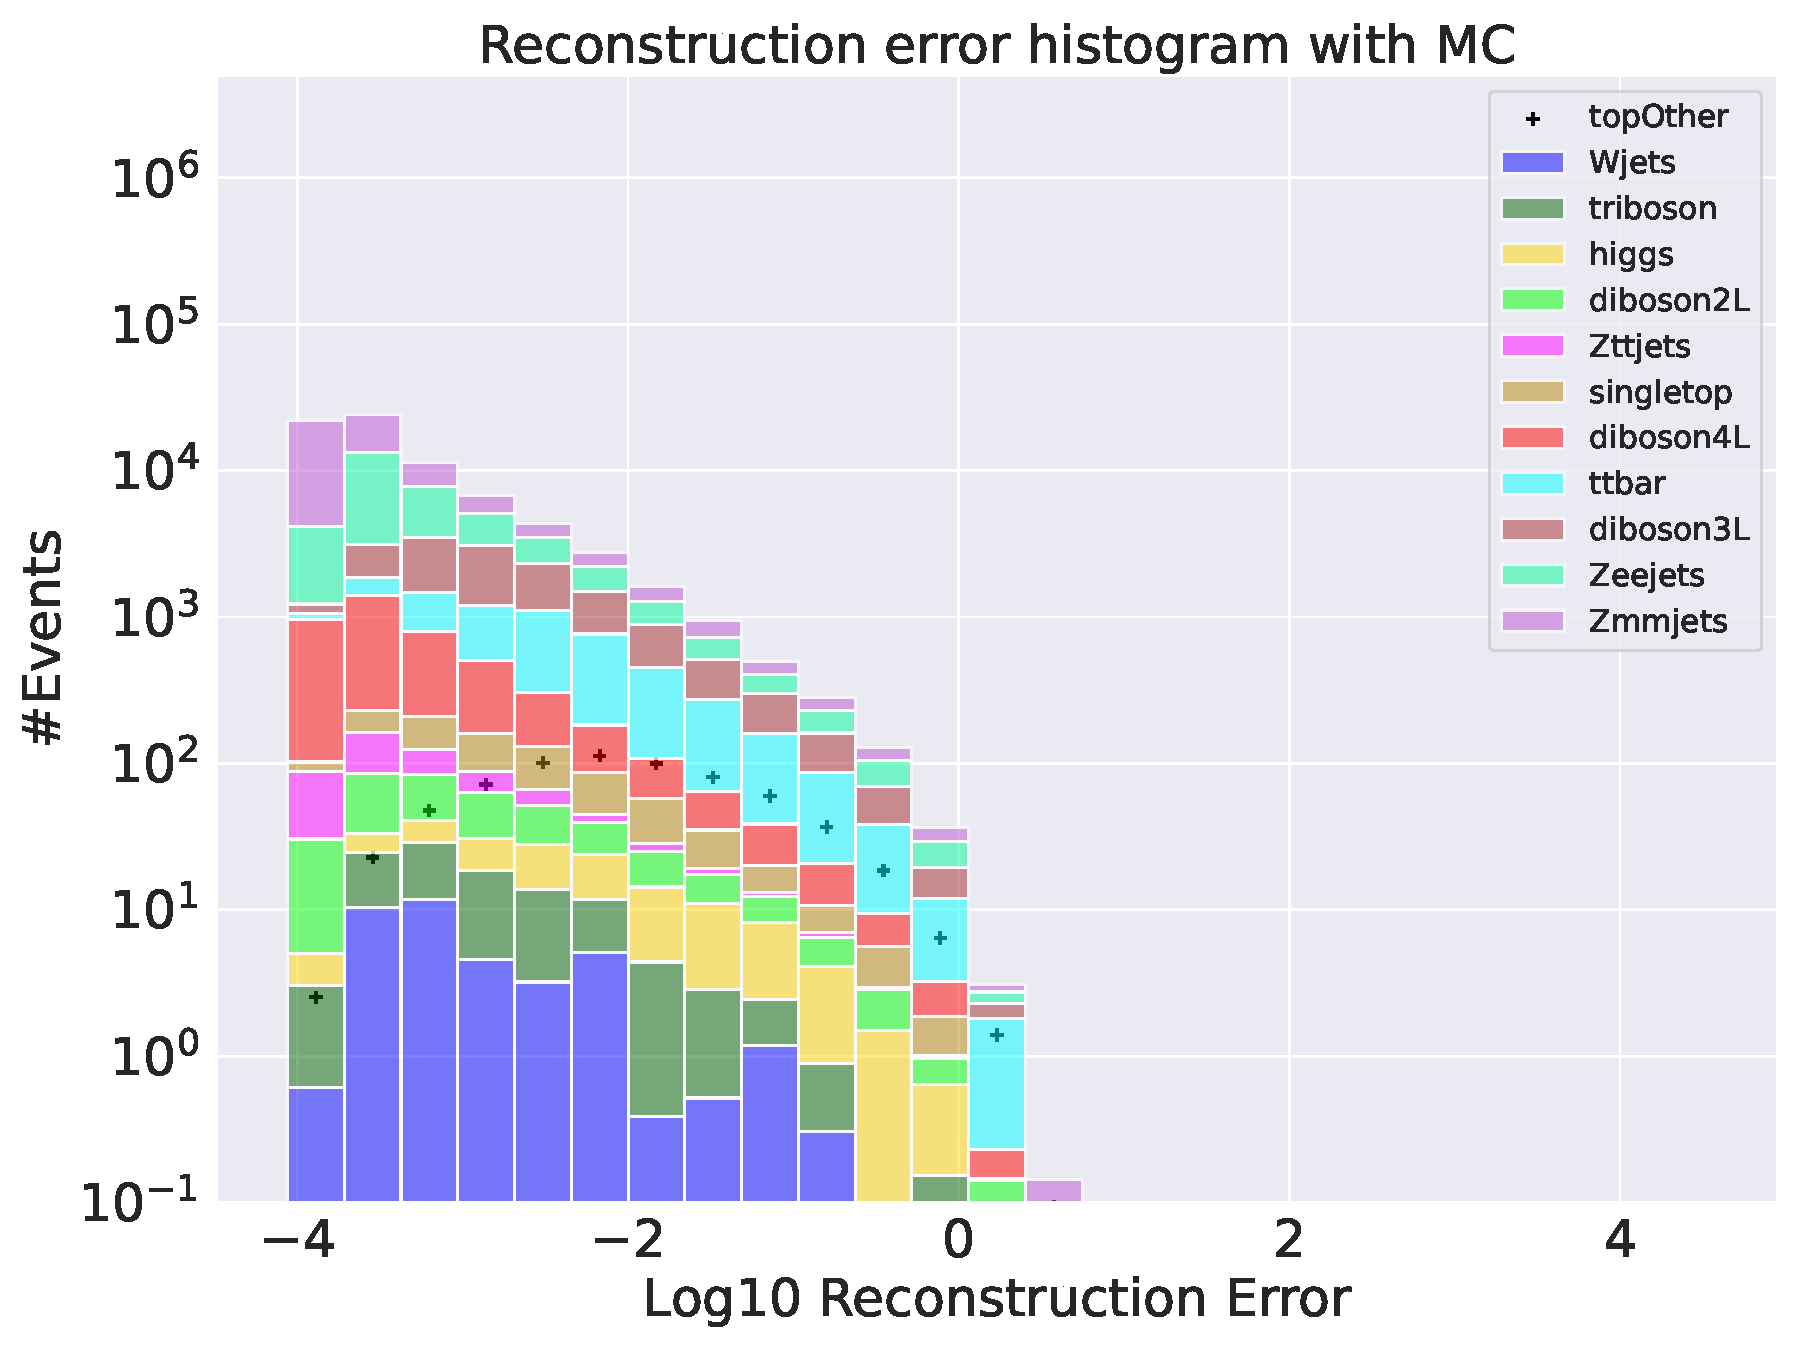
\includegraphics[width=\textwidth]{Figures/AE_testing/small/b_data_recon_big_rm3_feats_sig_topOther.pdf}
        \caption{Reconstruction error on validation SM MC from the Autoencoder. Here the topother channel has been removed from training and 
        is used as signal. No significant difference in distributions are found. }
        \label{fig:ae_small_topOther}
    \end{subfigure}
    \hfill        
    \caption{ }
    \label{fig:ae_small_channel3}
\end{figure}


\begin{figure}[h!]
    \centering
    \begin{subfigure}{.8\textwidth}
        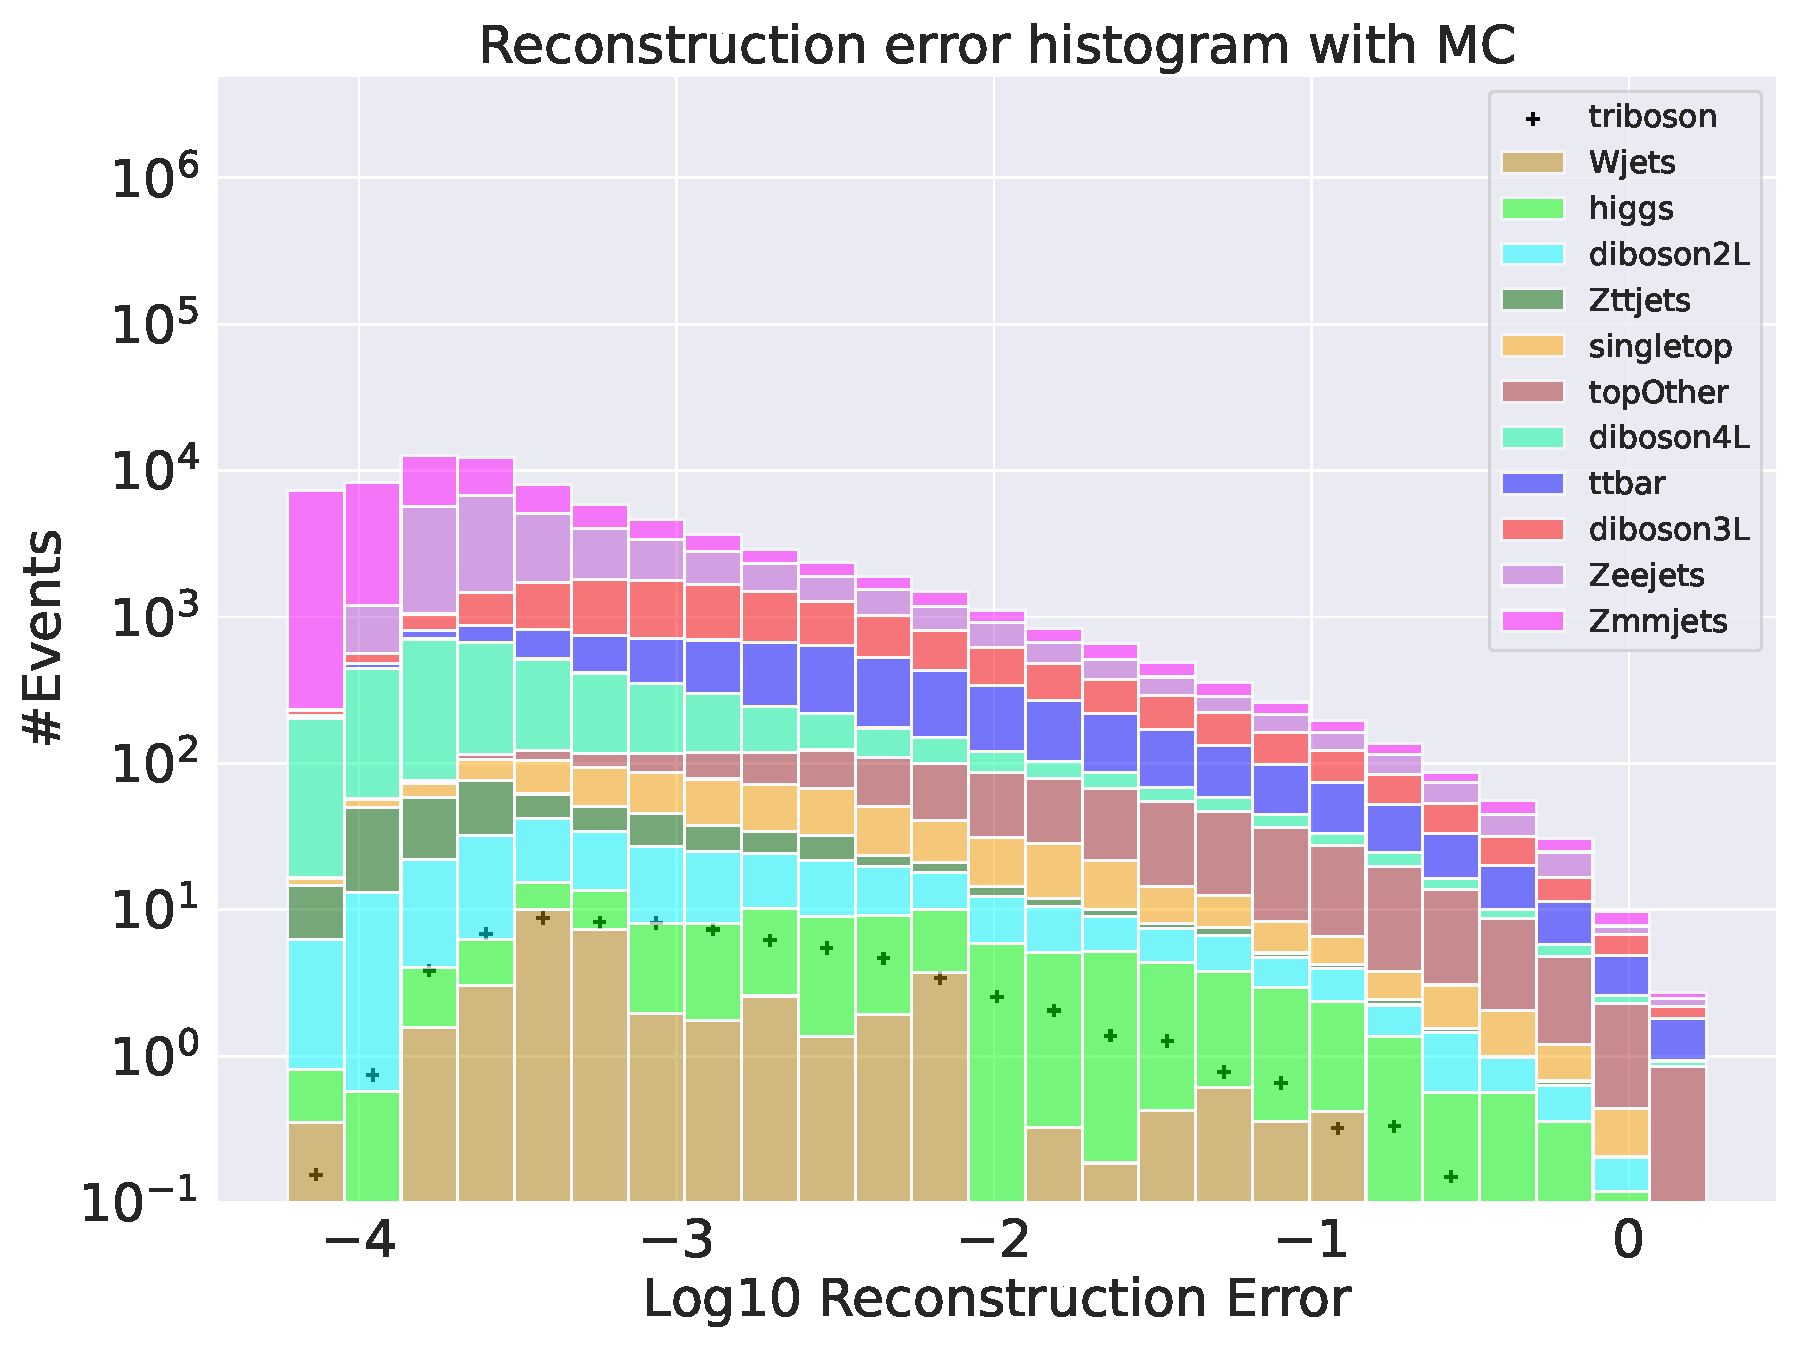
\includegraphics[width=\textwidth]{Figures/AE_testing/small/b_data_recon_big_rm3_feats_sig_triboson.pdf}
        \caption{Reconstruction error on validation SM MC from the Autoencoder. Here the triboson channel has been removed from training and 
        is used as signal. No significant difference in distributions are found. }
        \label{fig:ae_small_triboson}
    \end{subfigure}
    \hfill
    \begin{subfigure}{.8\textwidth}
        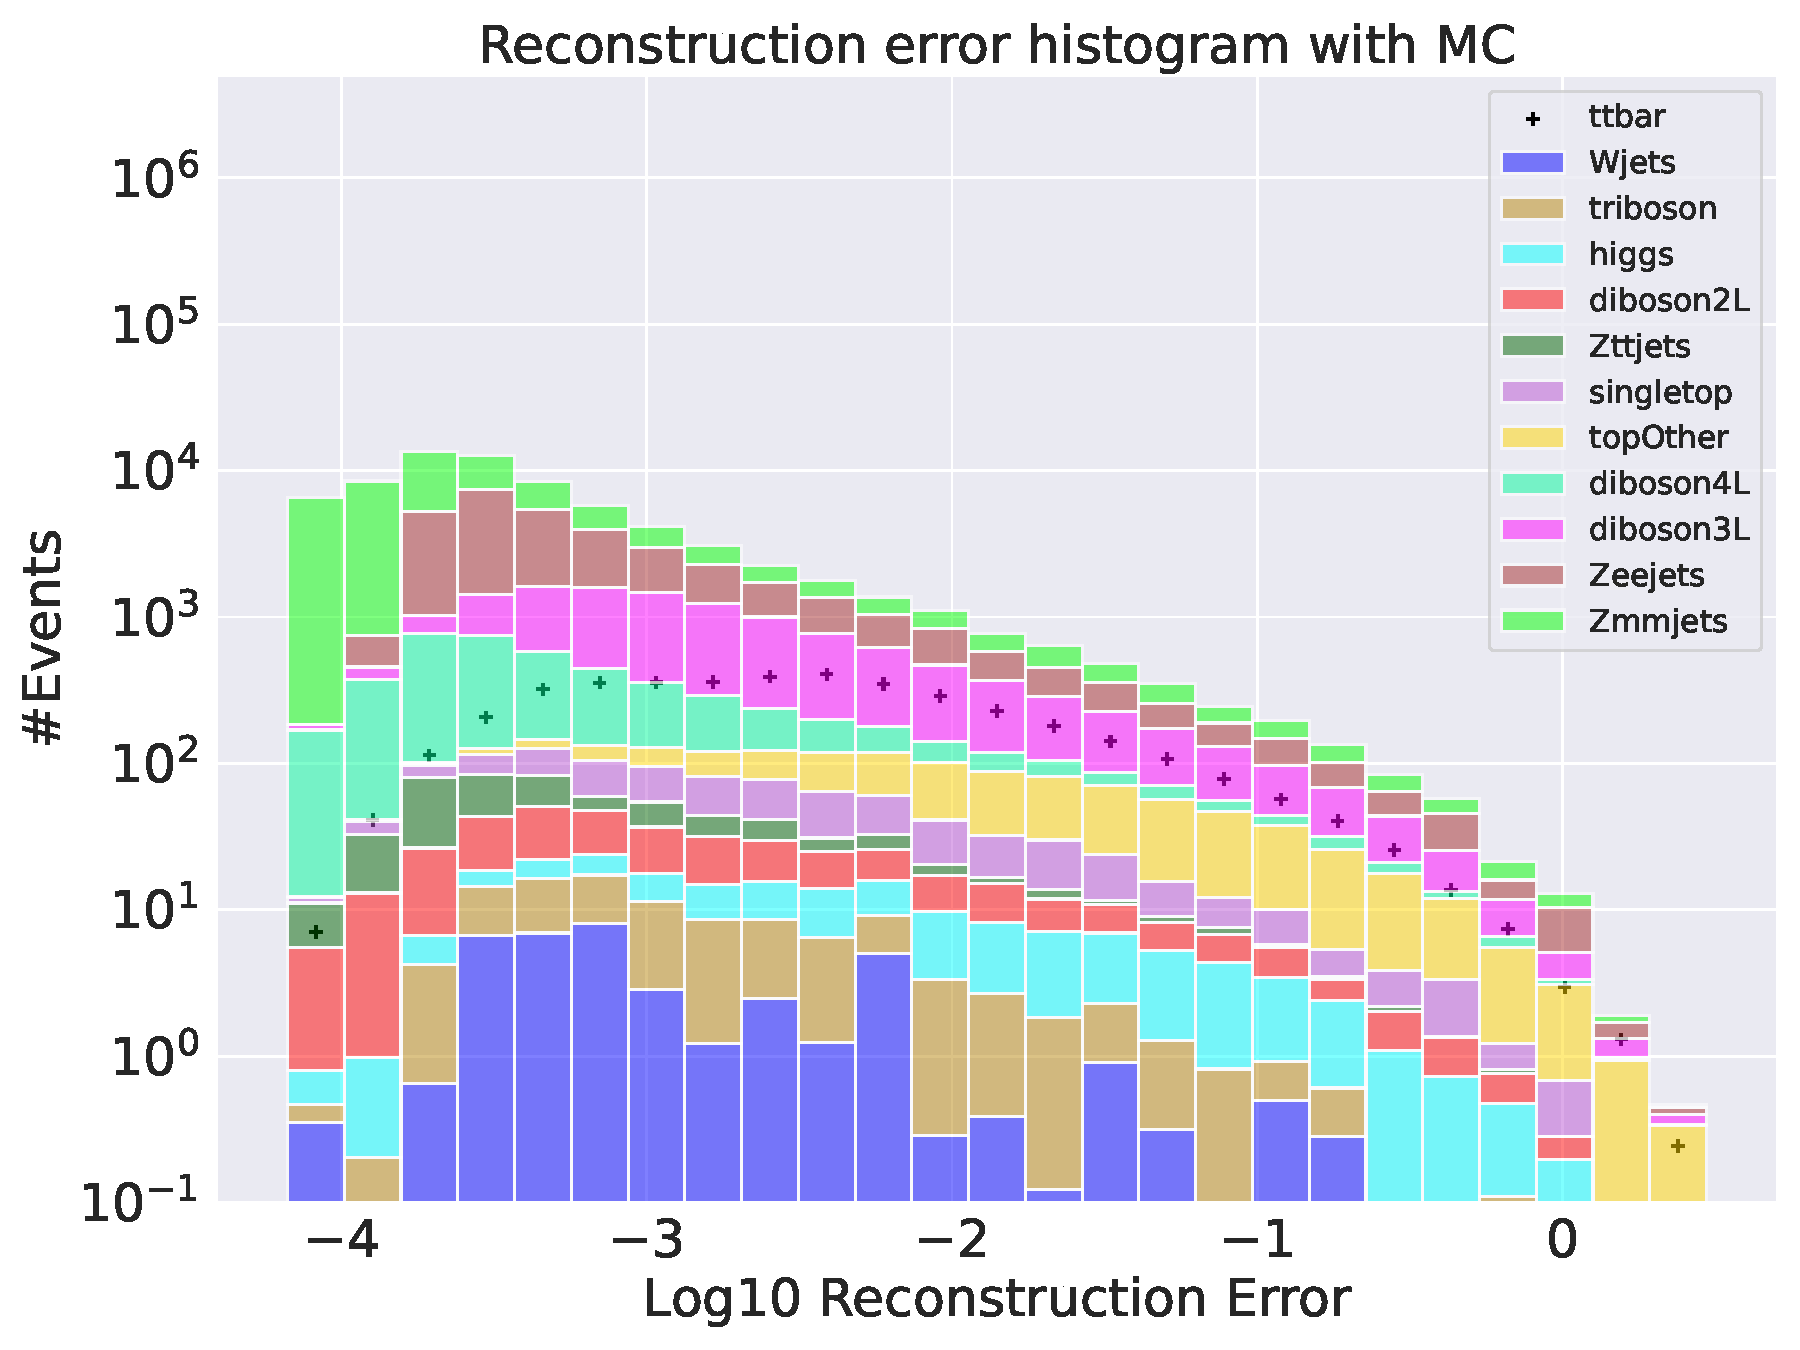
\includegraphics[width=\textwidth]{Figures/AE_testing/small/b_data_recon_big_rm3_feats_sig_ttbar.pdf}
        \caption{Reconstruction error on validation SM MC from the Autoencoder. Here the ttbar channel has been removed from training and 
        is used as signal. No significant difference in distributions are found. }
        \label{fig:ae_small_ttbar}
    \end{subfigure}
    \hfill        
    \caption{ }
    \label{fig:ae_small_channel4}
\end{figure}

\begin{figure}[h!]
    \centering
    \begin{subfigure}{.8\textwidth}
        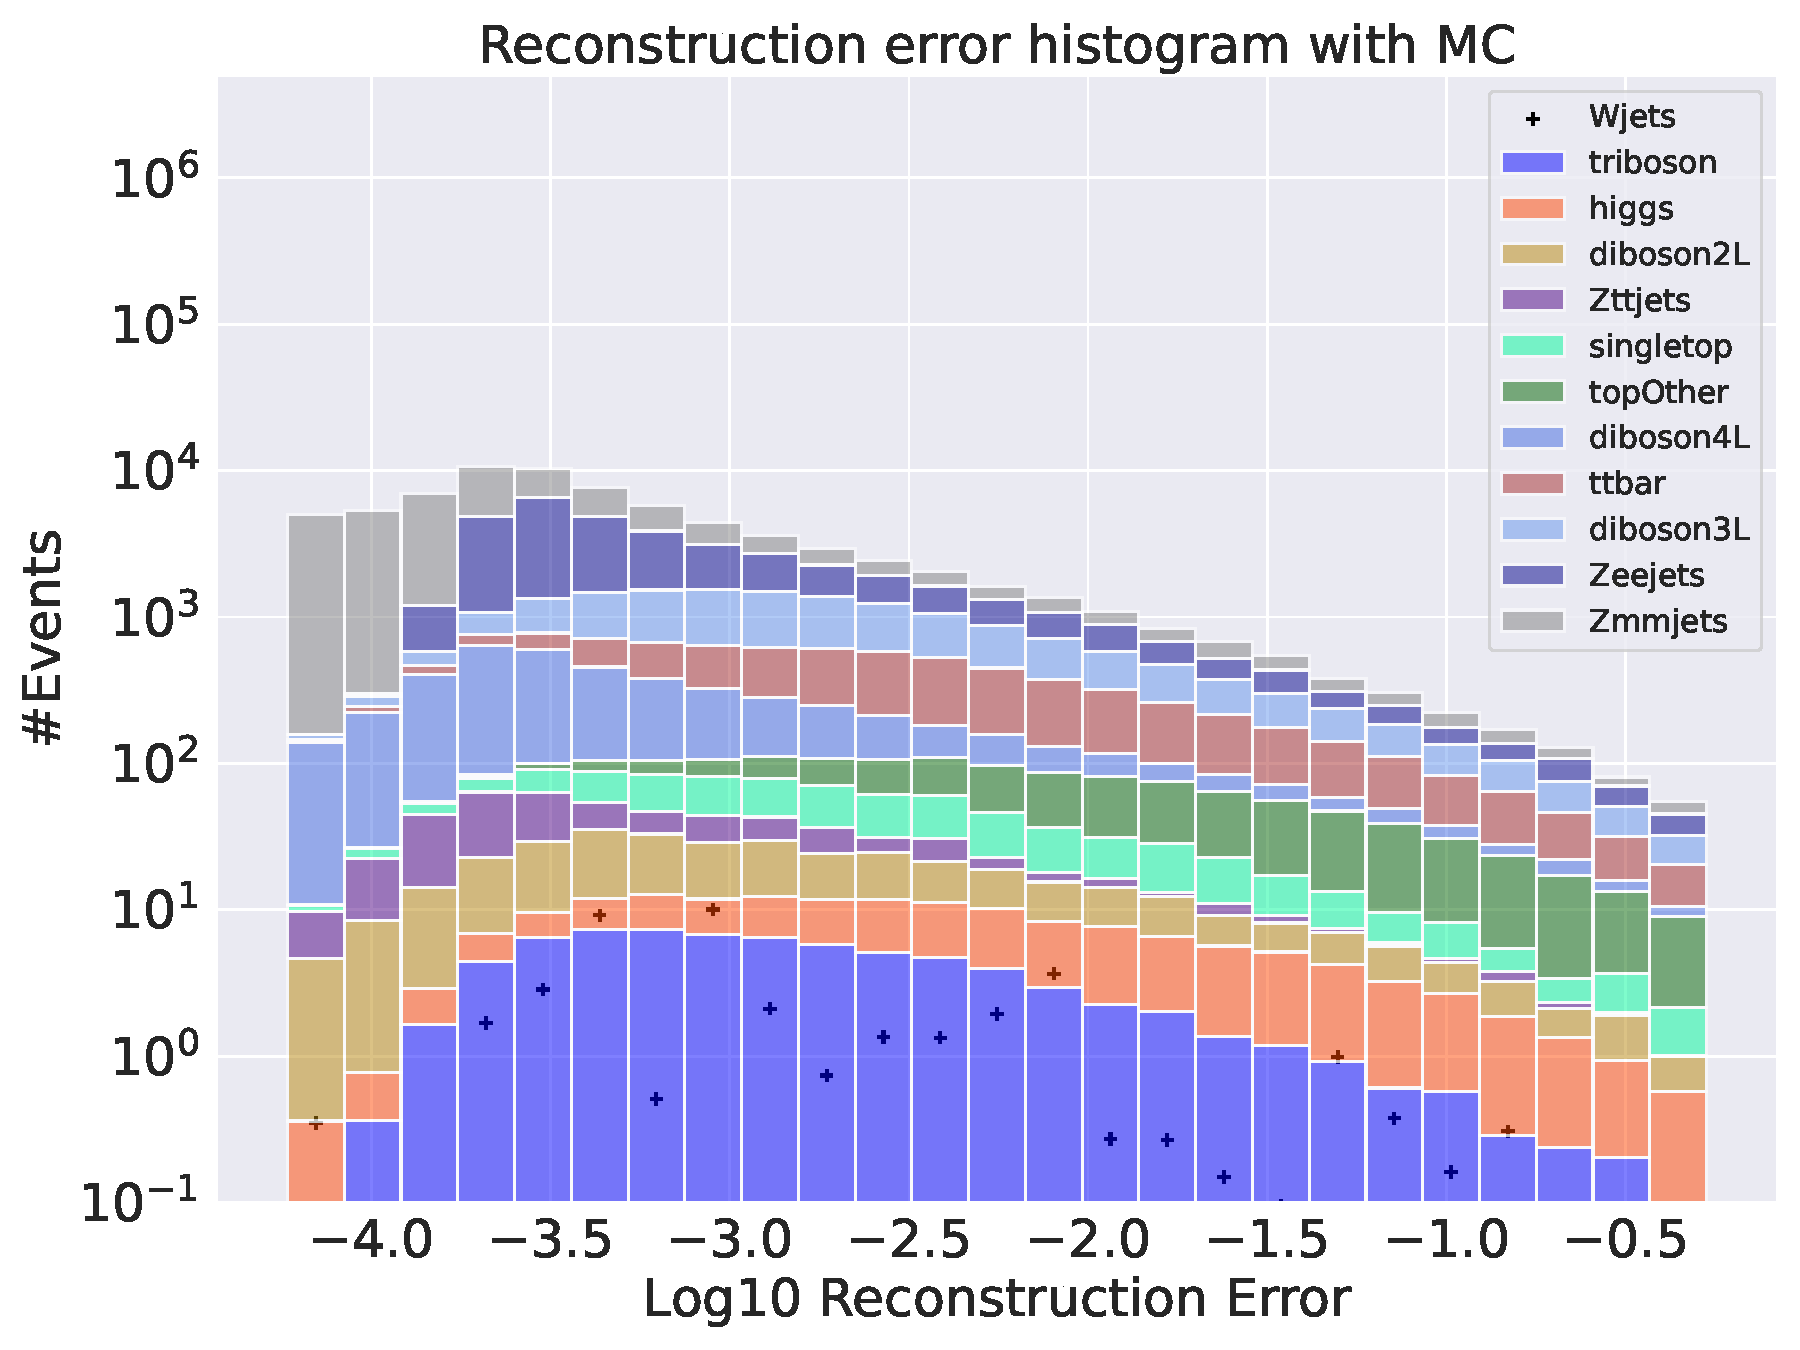
\includegraphics[width=\textwidth]{Figures/AE_testing/small/b_data_recon_big_rm3_feats_sig_Wjets.pdf}
        \caption{Reconstruction error on validation SM MC from the Autoencoder. Here the wjets channel has been removed from training and 
        is used as signal. No significant difference in distributions are found. }
        \label{fig:ae_small_wjets}
    \end{subfigure}
    \hfill
    \begin{subfigure}{.8\textwidth}
        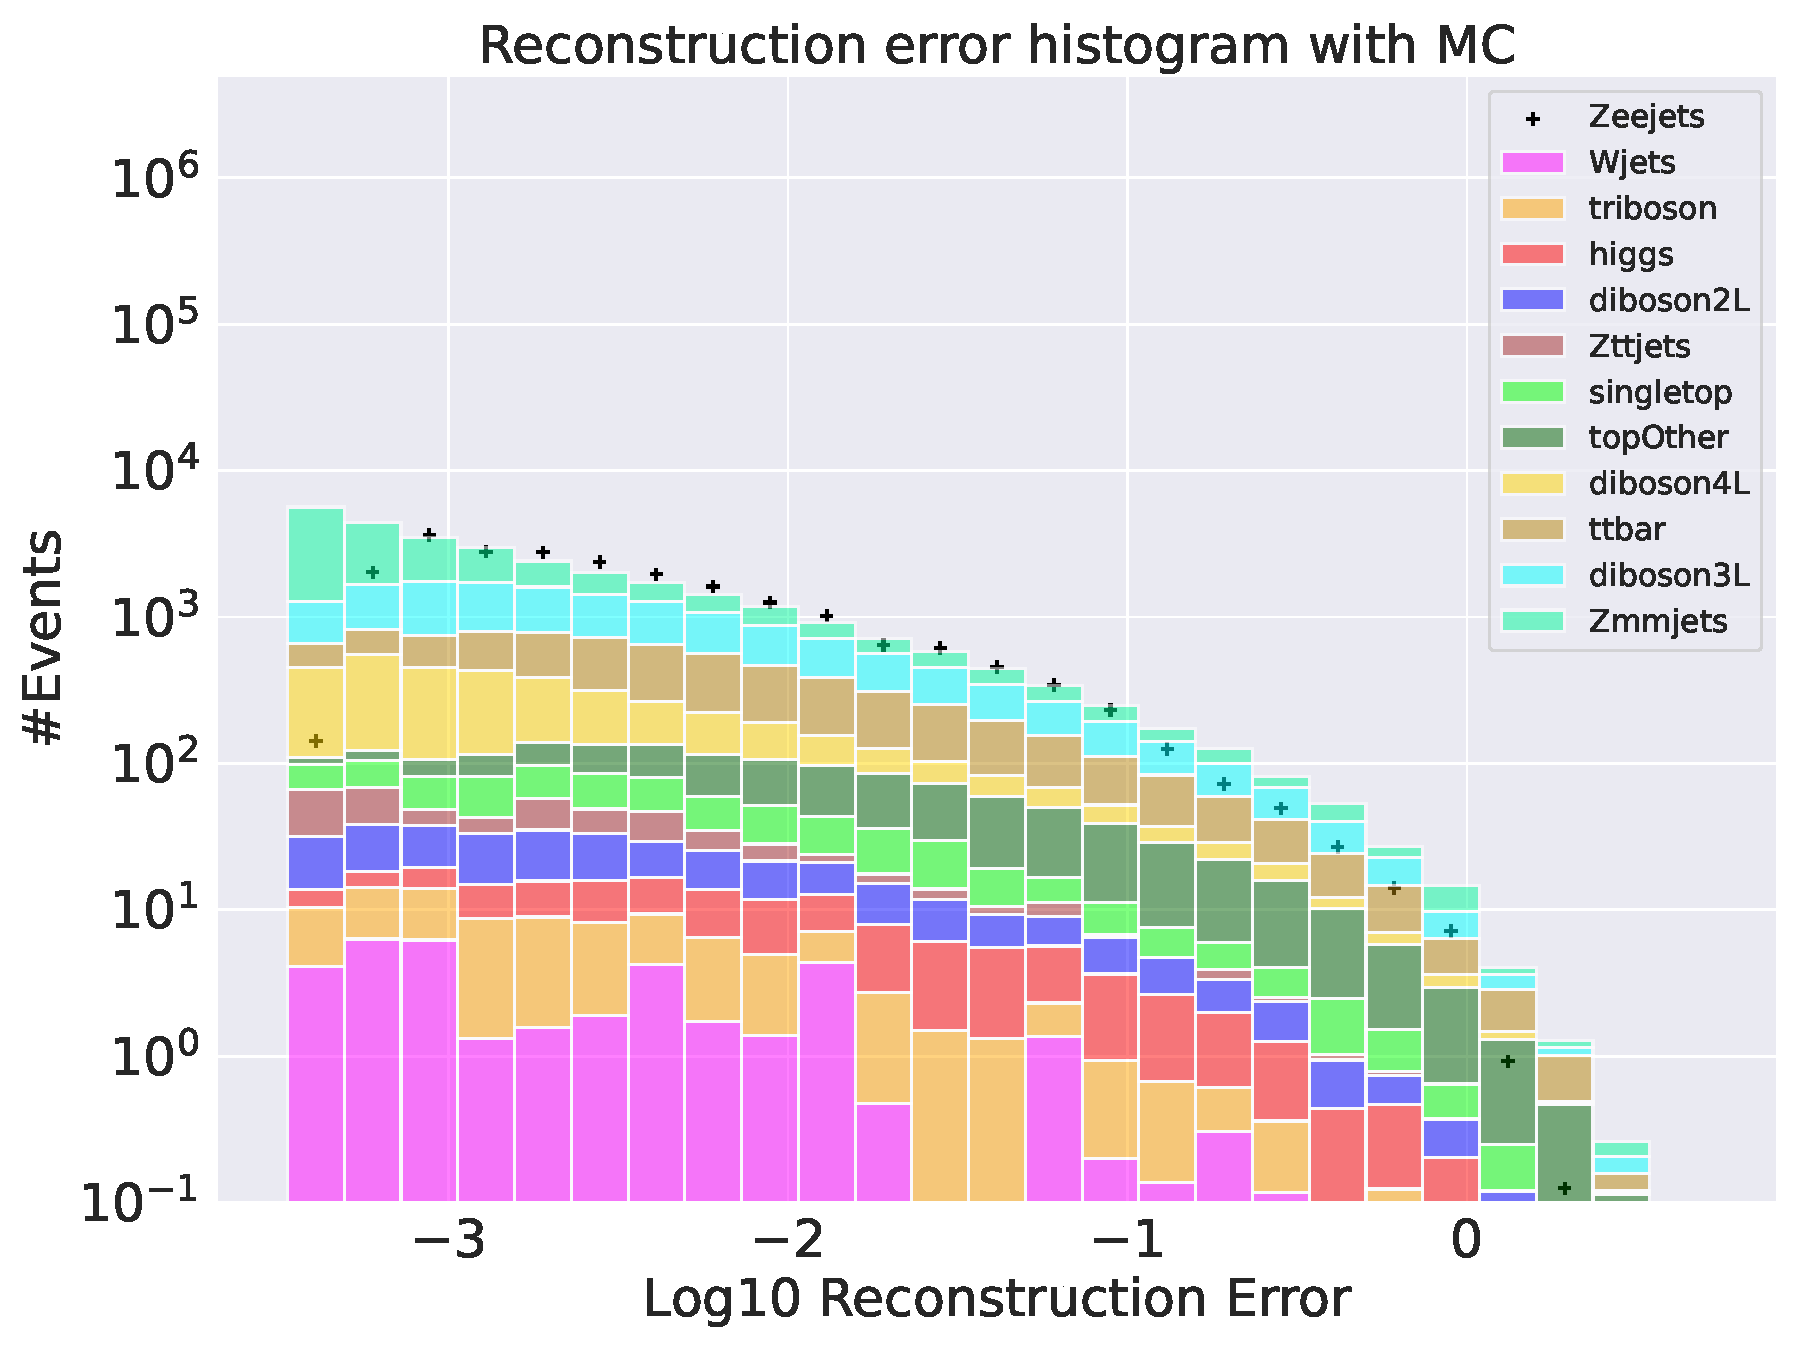
\includegraphics[width=\textwidth]{Figures/AE_testing/small/b_data_recon_big_rm3_feats_sig_Zeejets.pdf}
        \caption{Reconstruction error on validation SM MC from the Autoencoder. Here the zeejets channel has been removed from training and 
        is used as signal. No significant difference in distributions are found. }
        \label{fig:ae_small_zeejets}
    \end{subfigure}
    \hfill        
    \caption{ }
    \label{fig:ae_small_channel5}
\end{figure}

\begin{figure}[h!]
    \centering
    \begin{subfigure}{.8\textwidth}
        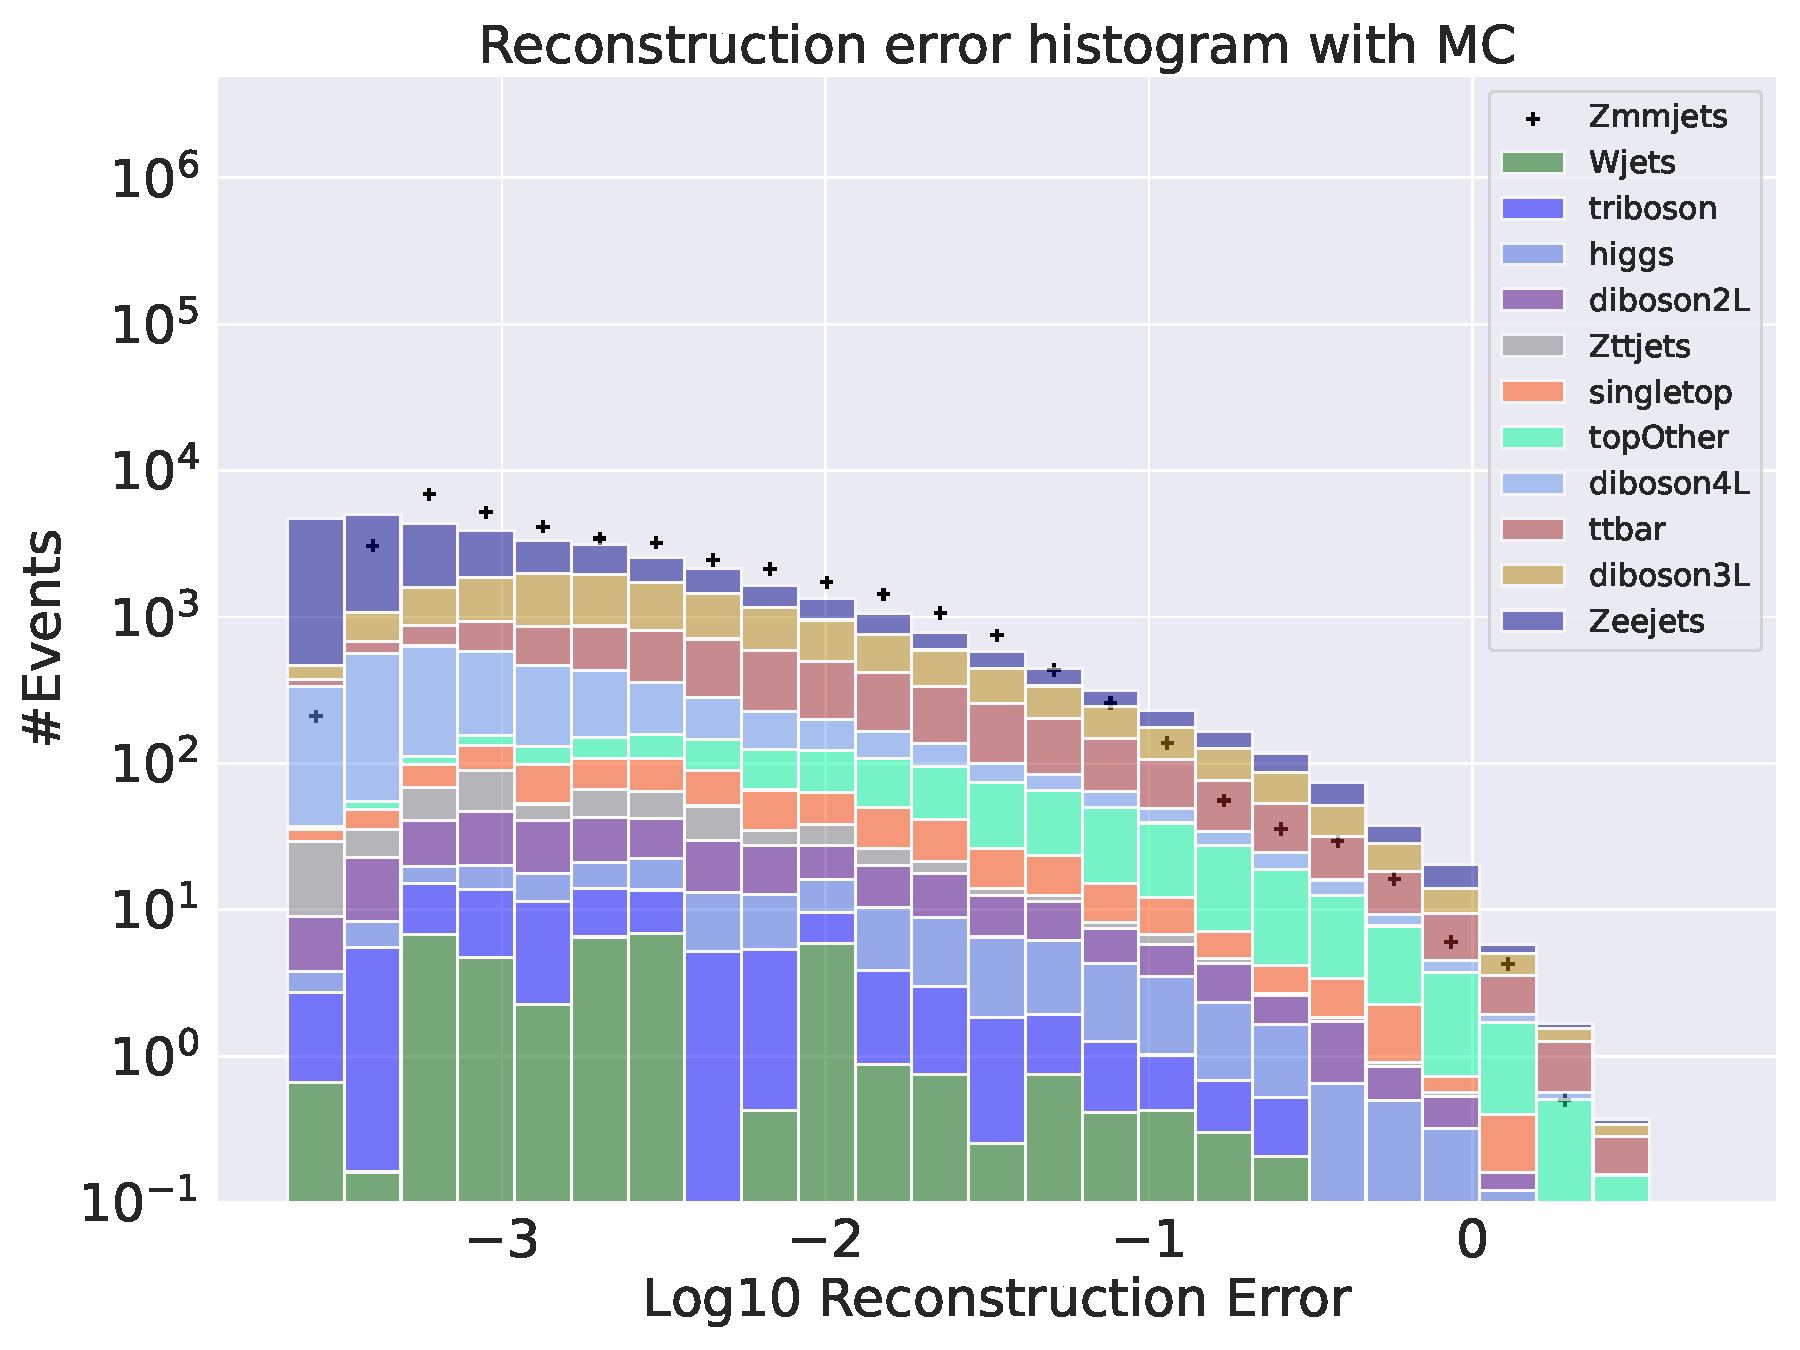
\includegraphics[width=\textwidth]{Figures/AE_testing/small/b_data_recon_big_rm3_feats_sig_Zmmjets.pdf}
        \caption{Reconstruction error on validation SM MC from the Autoencoder. Here the zmmjets channel has been removed from training and 
        is used as signal. No significant difference in distributions are found.  }
        \label{fig:ae_small_zmmjets}
    \end{subfigure}
    \hfill
    \begin{subfigure}{.8\textwidth}
        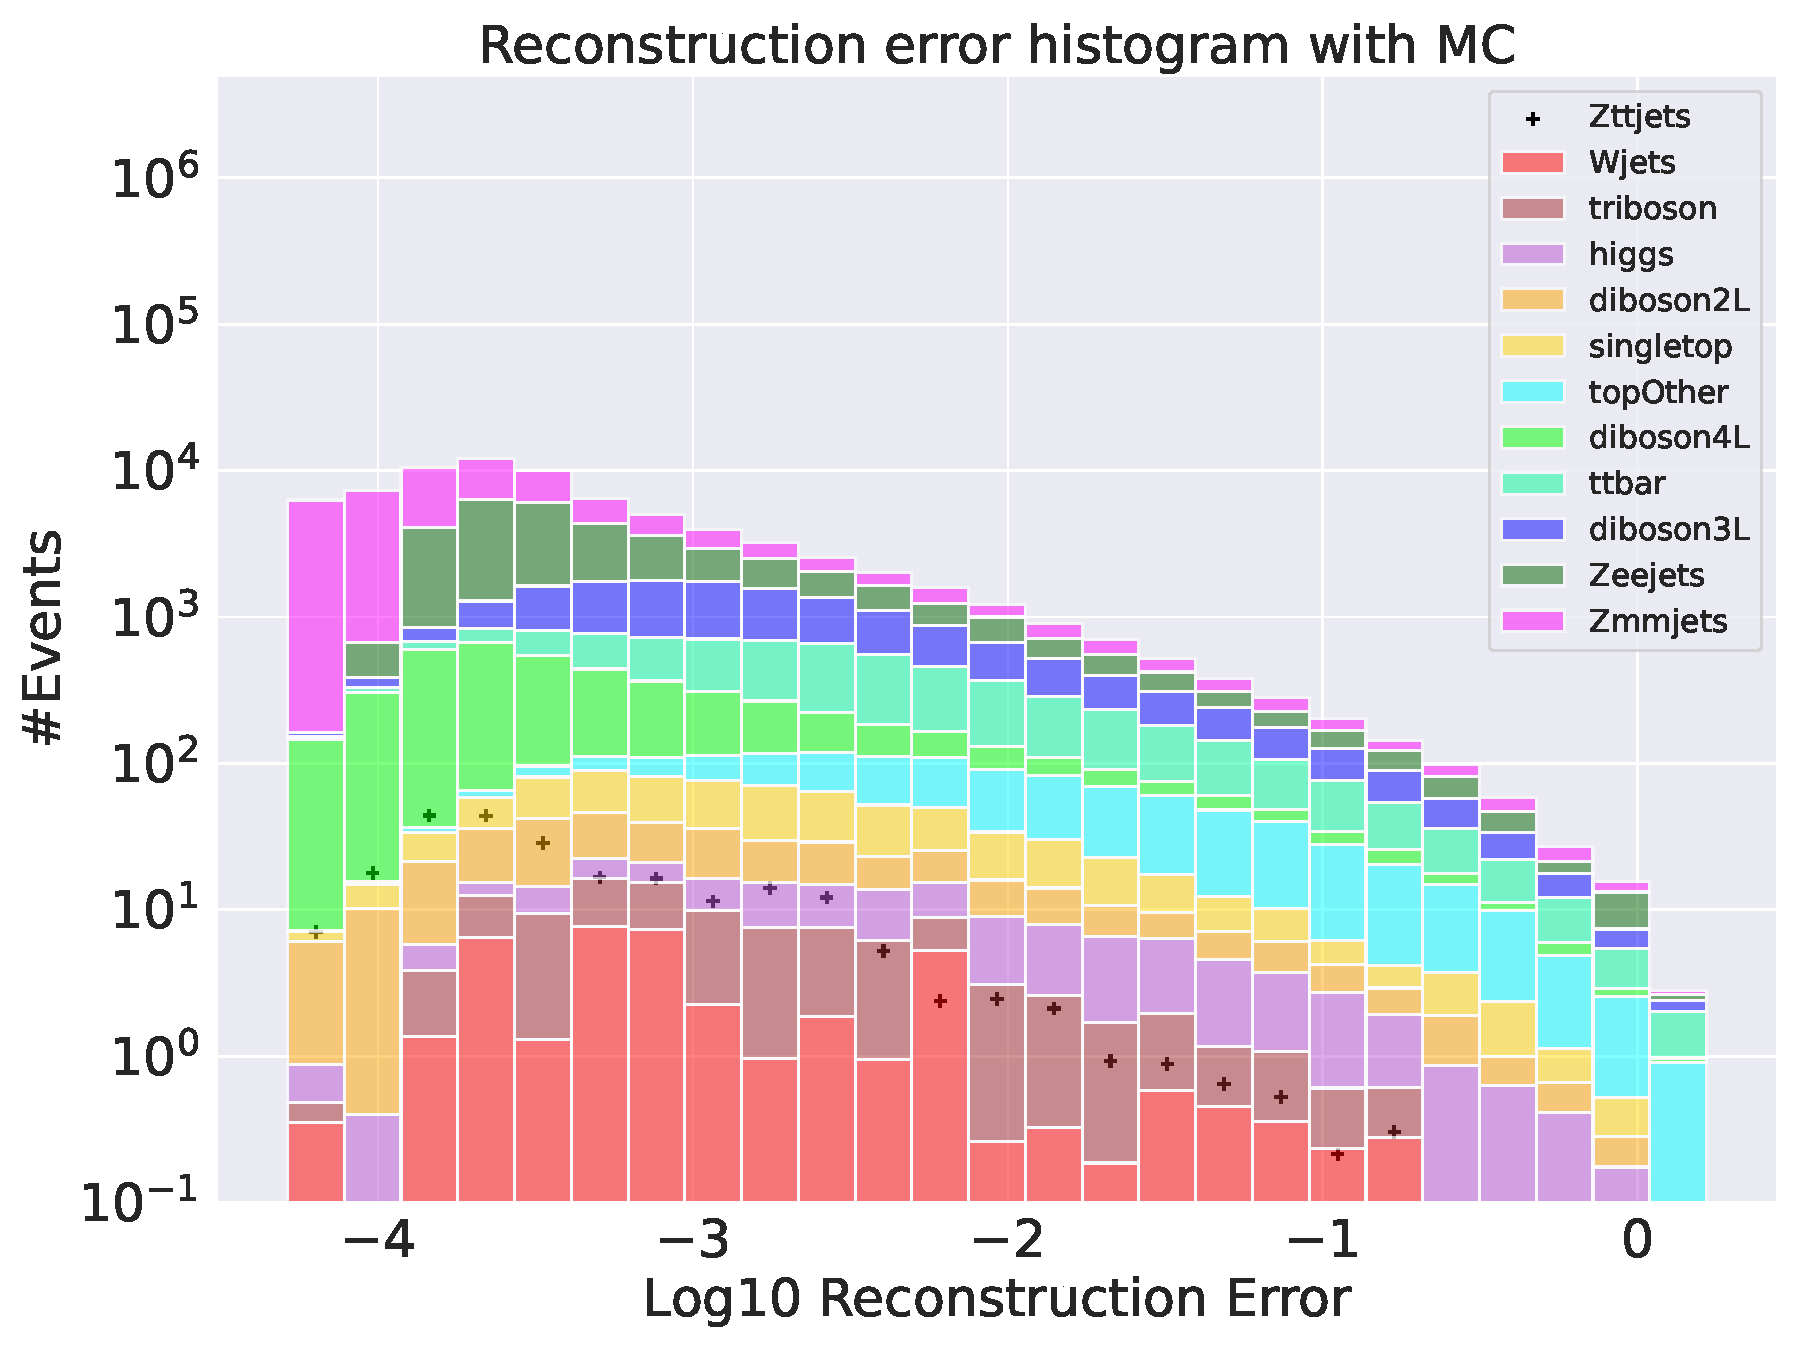
\includegraphics[width=\textwidth]{Figures/AE_testing/small/b_data_recon_big_rm3_feats_sig_Zttjets.pdf}
        \caption{Reconstruction error on validation SM MC from the Autoencoder. Here the zttjets channel has been removed from training and 
        is used as signal. No significant difference in distributions are found. }
        \label{fig:ae_small_zttjets}
    \end{subfigure}
    \hfill        
    \caption{ }
    \label{fig:ae_small_channel6}
\end{figure}


Big autoencoder

\begin{figure}[h!]
    \centering
    \begin{subfigure}{.8\textwidth}
        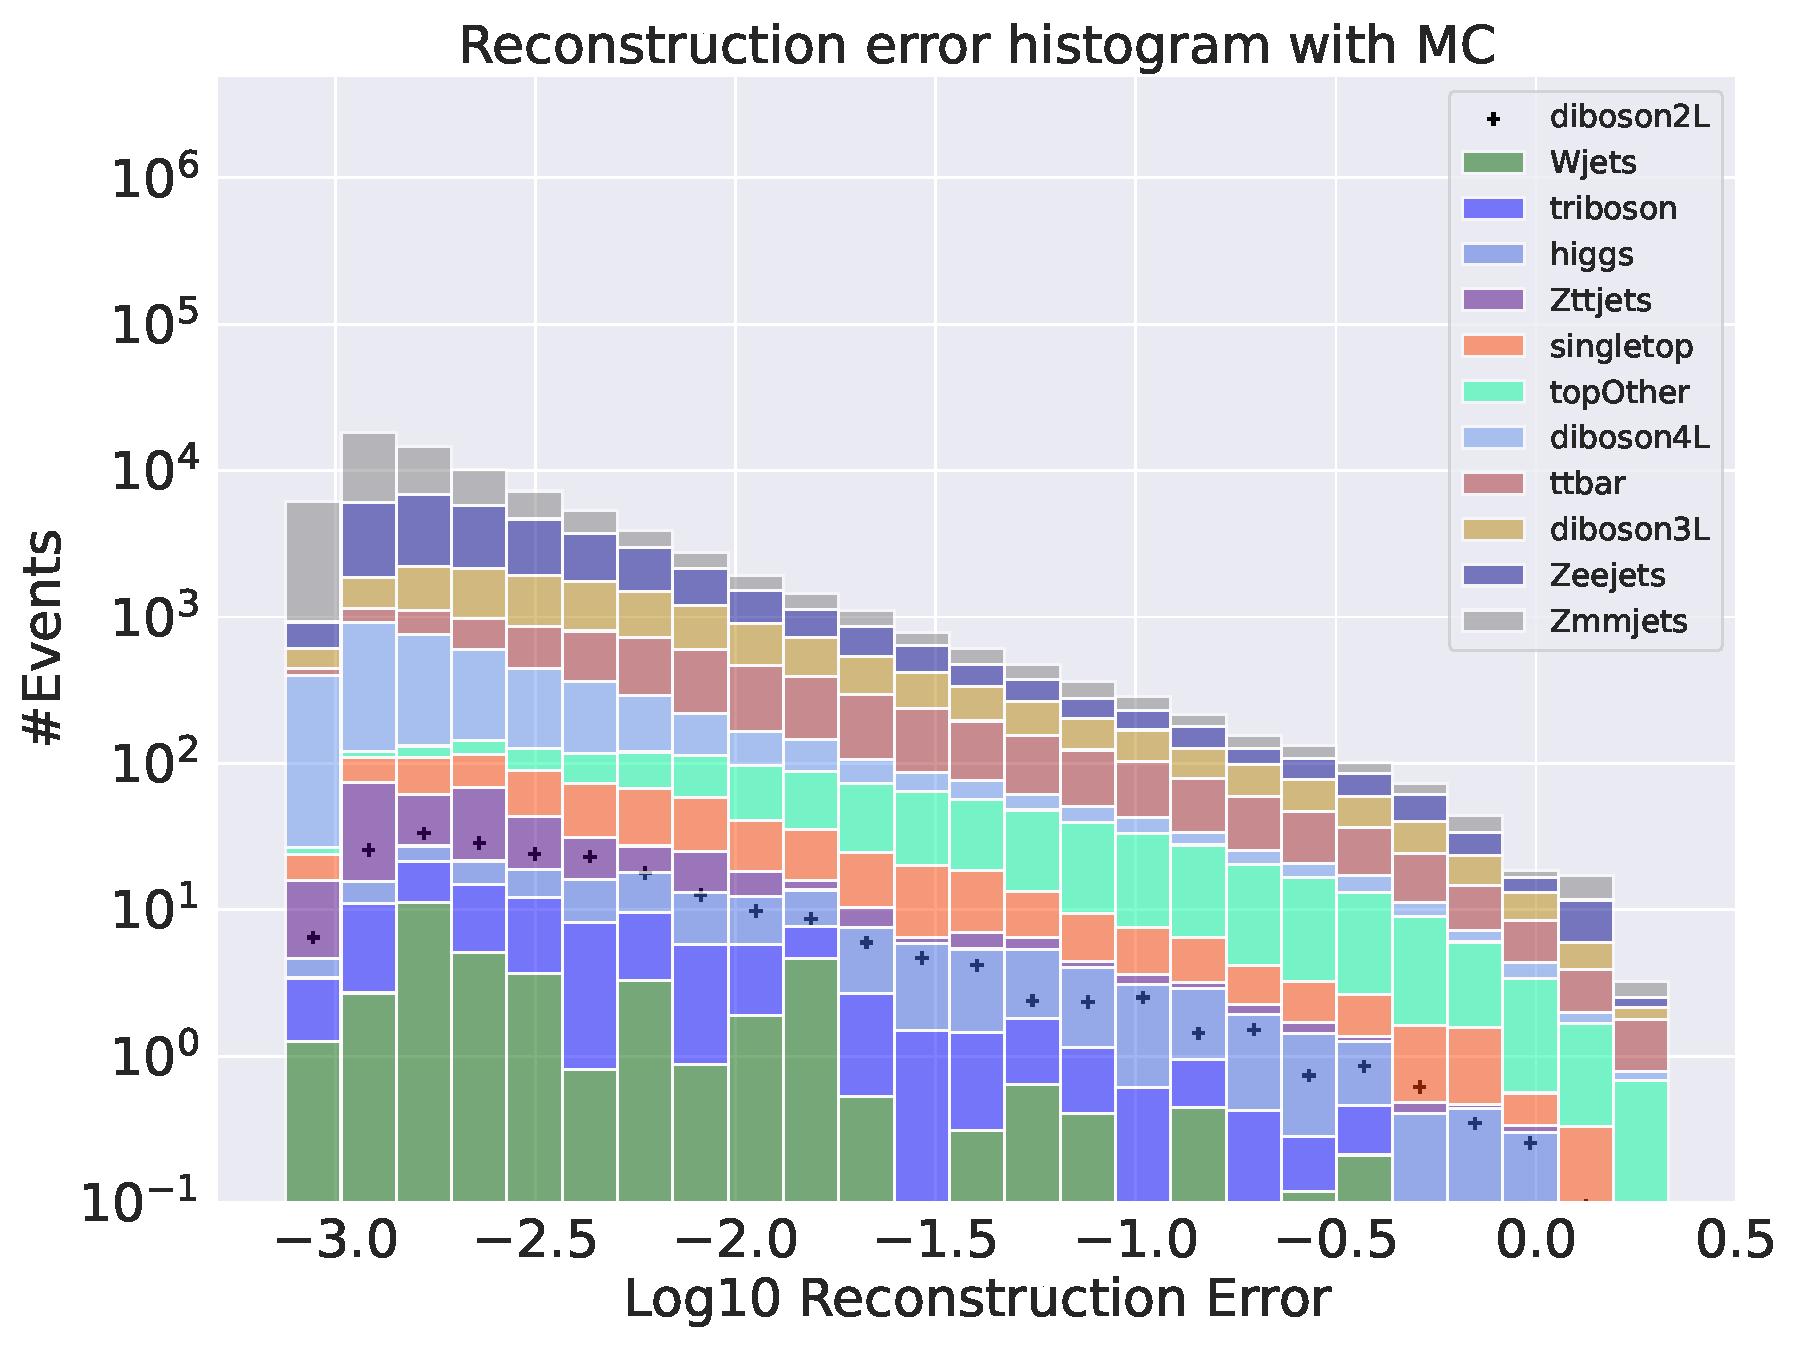
\includegraphics[width=\textwidth]{Figures/AE_testing/big/b_data_recon_big_rm3_feats_sig_diboson2L.pdf}
        \caption{Reconstruction error on validation SM MC from the Autoencoder. }
        \label{fig:ae_big_diboson2l}
    \end{subfigure}
    \hfill
    \begin{subfigure}{.8\textwidth}
        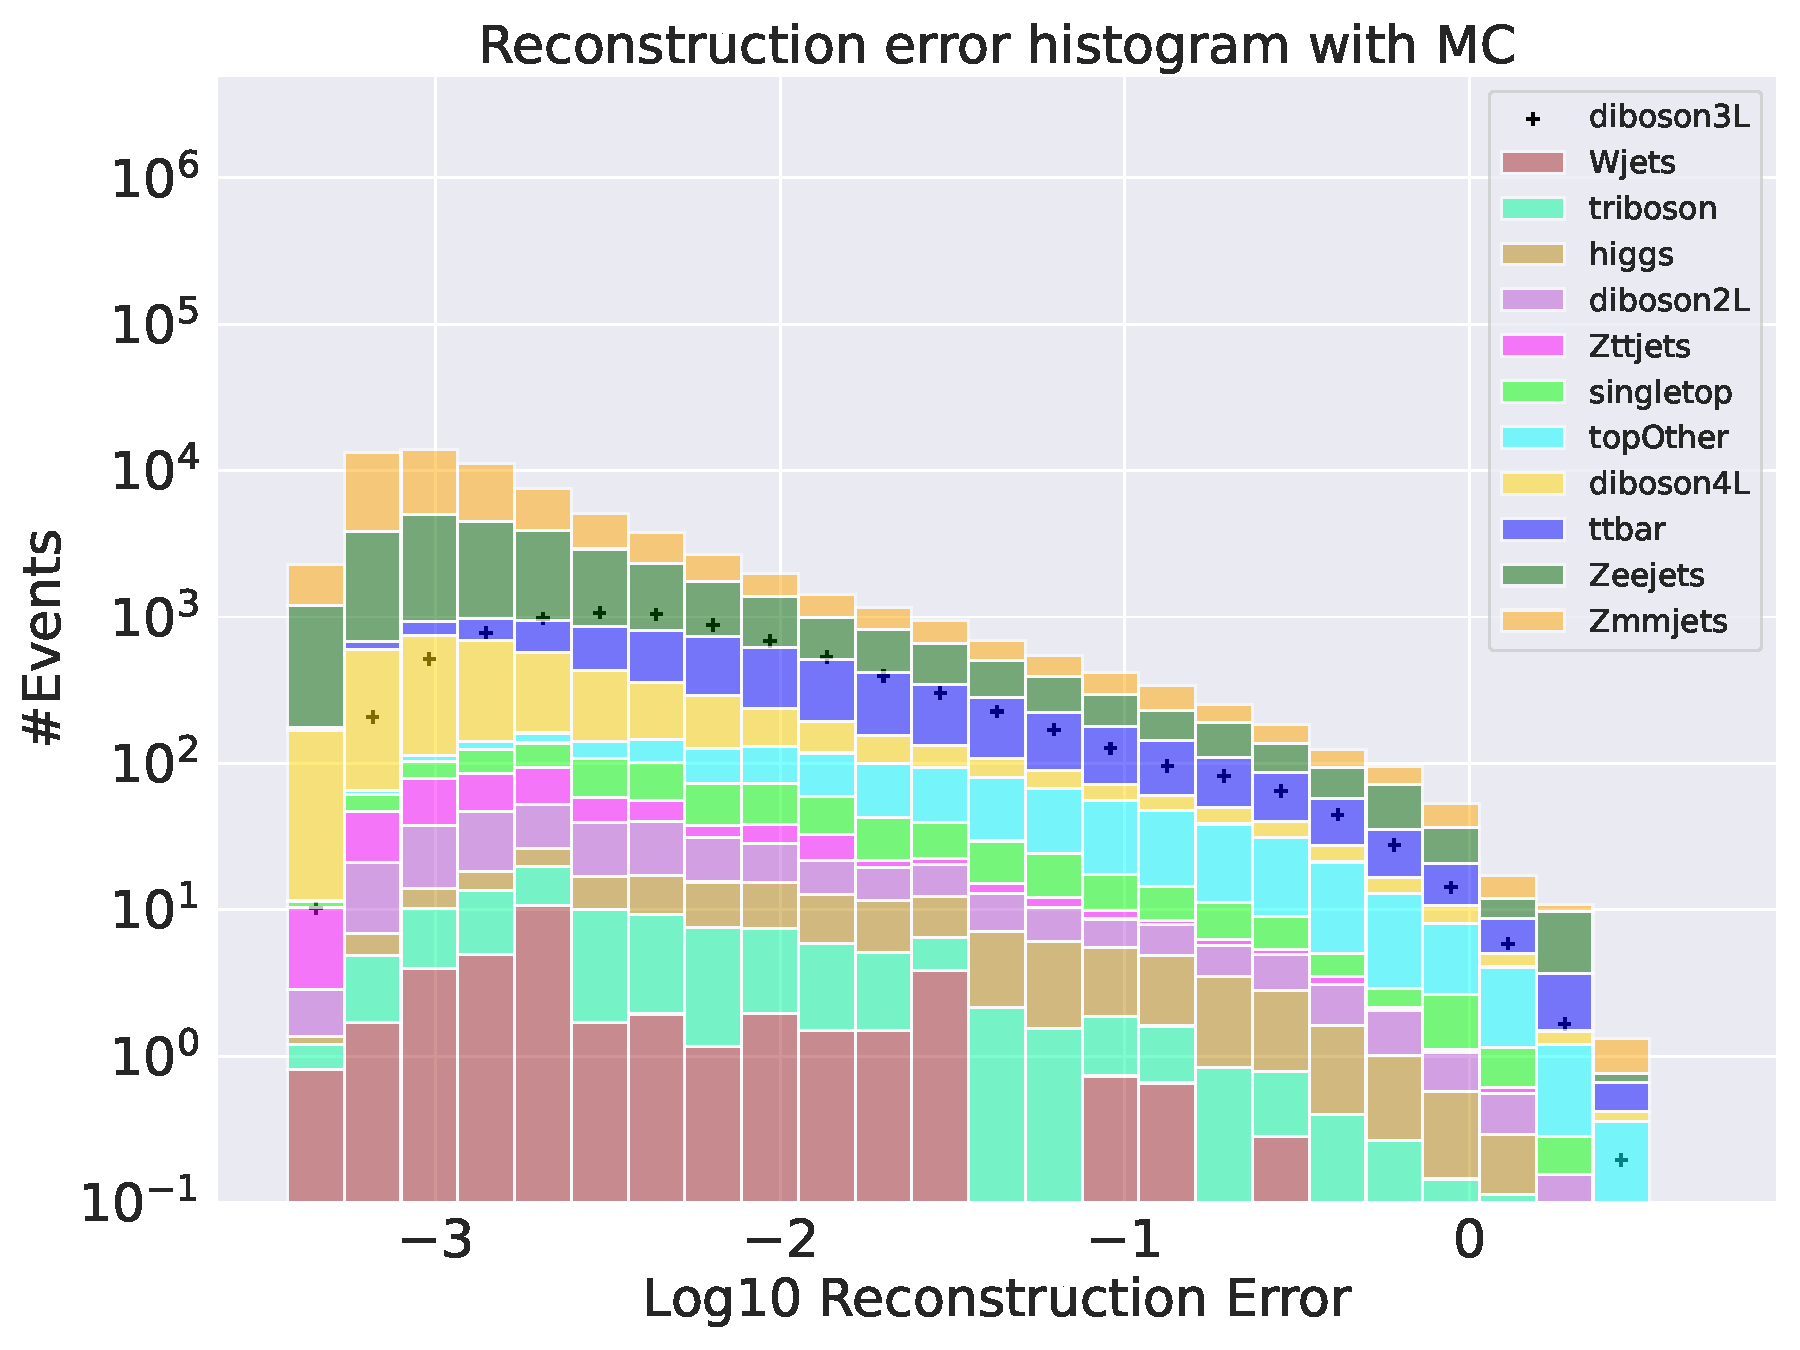
\includegraphics[width=\textwidth]{Figures/AE_testing/big/b_data_recon_big_rm3_feats_sig_diboson3L.pdf}
        \caption{}
        \label{fig:ae_big_diboson3l}
    \end{subfigure}
    \hfill        
    \caption{ }
    \label{fig:ae_big_channel1}
\end{figure}

\begin{figure}[h!]
    \centering
    \begin{subfigure}{.8\textwidth}
        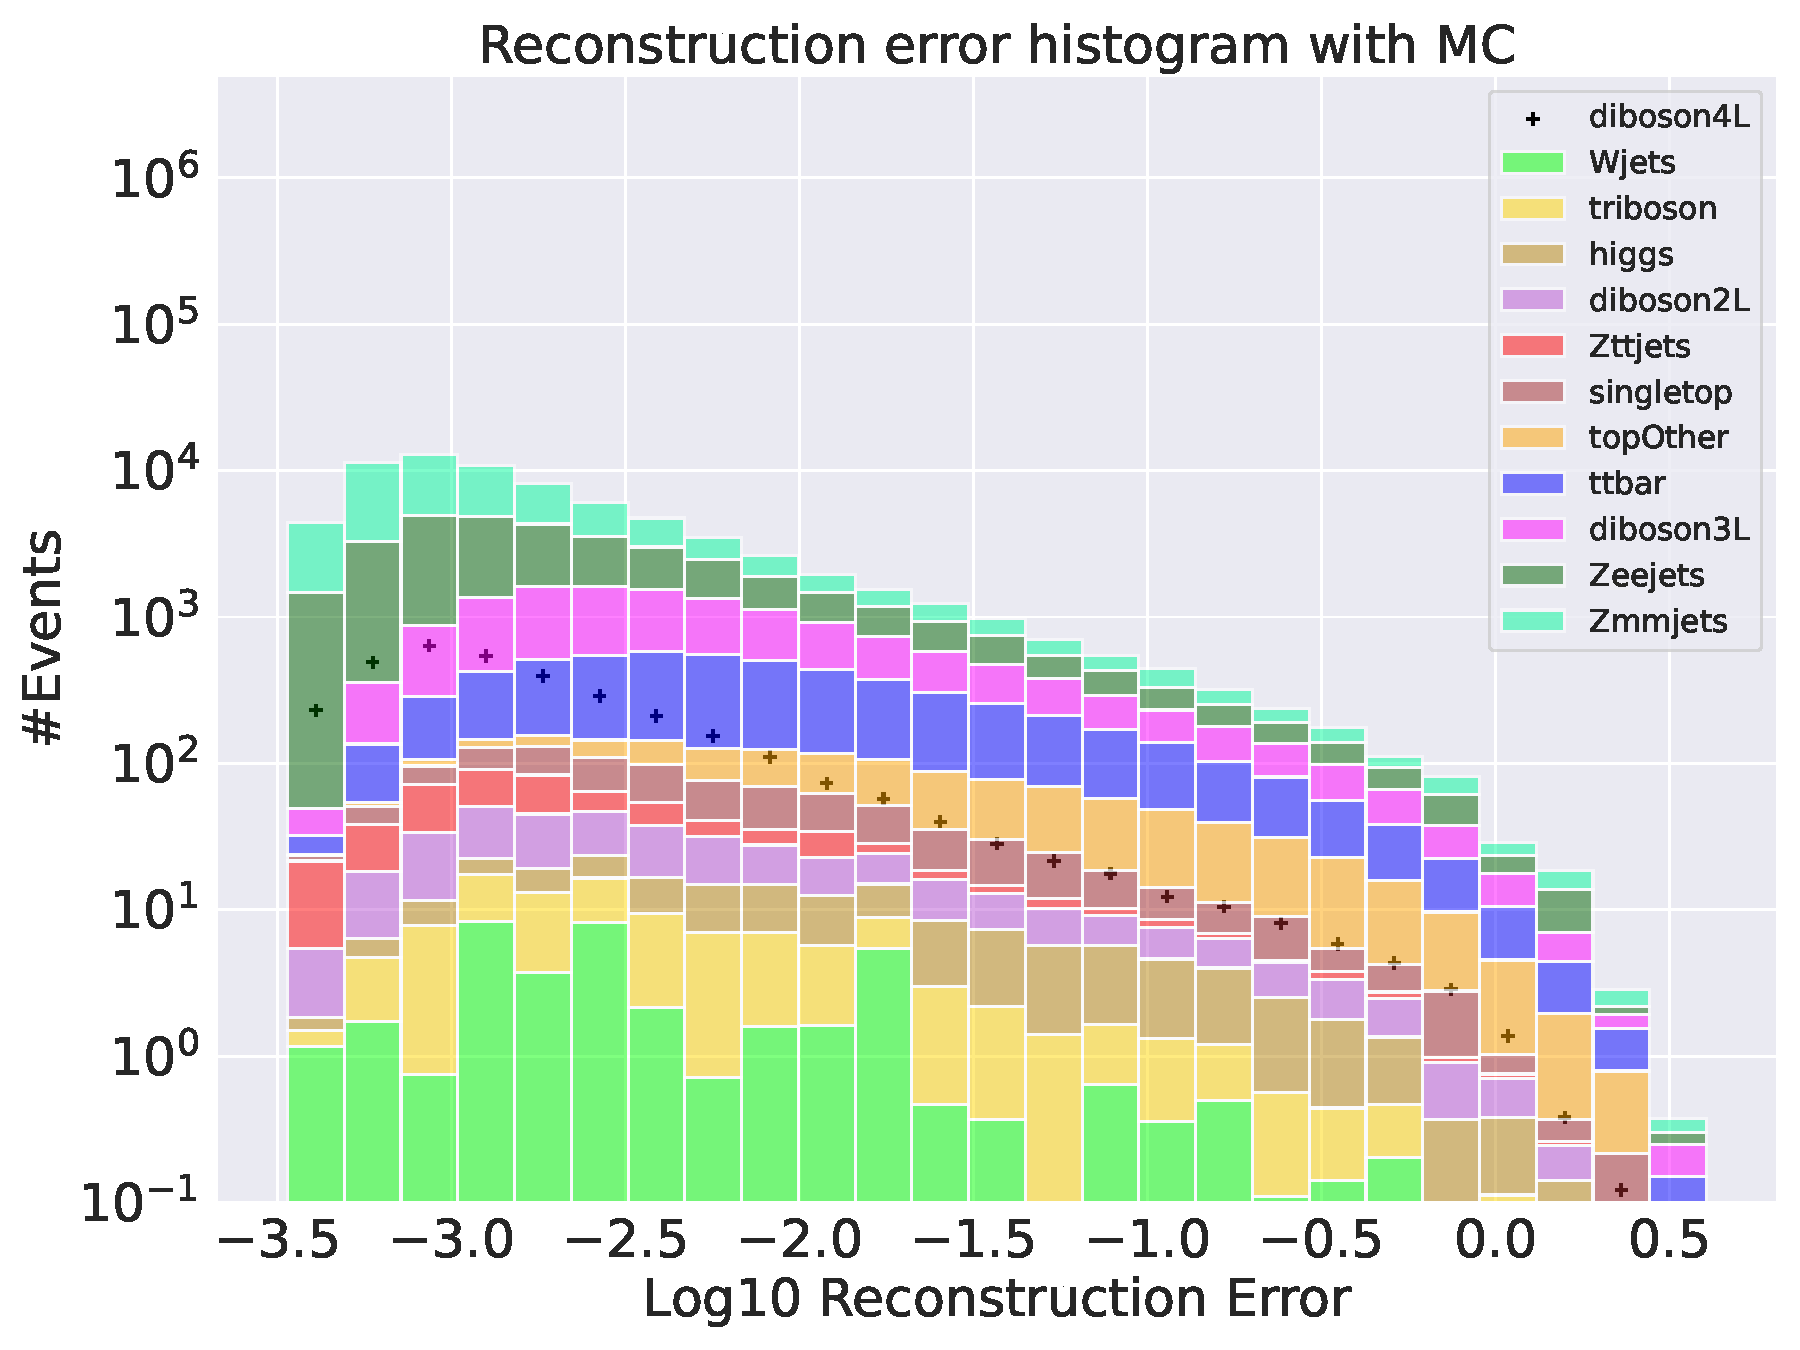
\includegraphics[width=\textwidth]{Figures/AE_testing/big/b_data_recon_big_rm3_feats_sig_diboson4L.pdf}
        \caption{Reconstruction error on validation SM MC from the Autoencoder. }
        \label{fig:ae_big_diboson4l}
    \end{subfigure}
    \hfill
    \begin{subfigure}{.8\textwidth}
        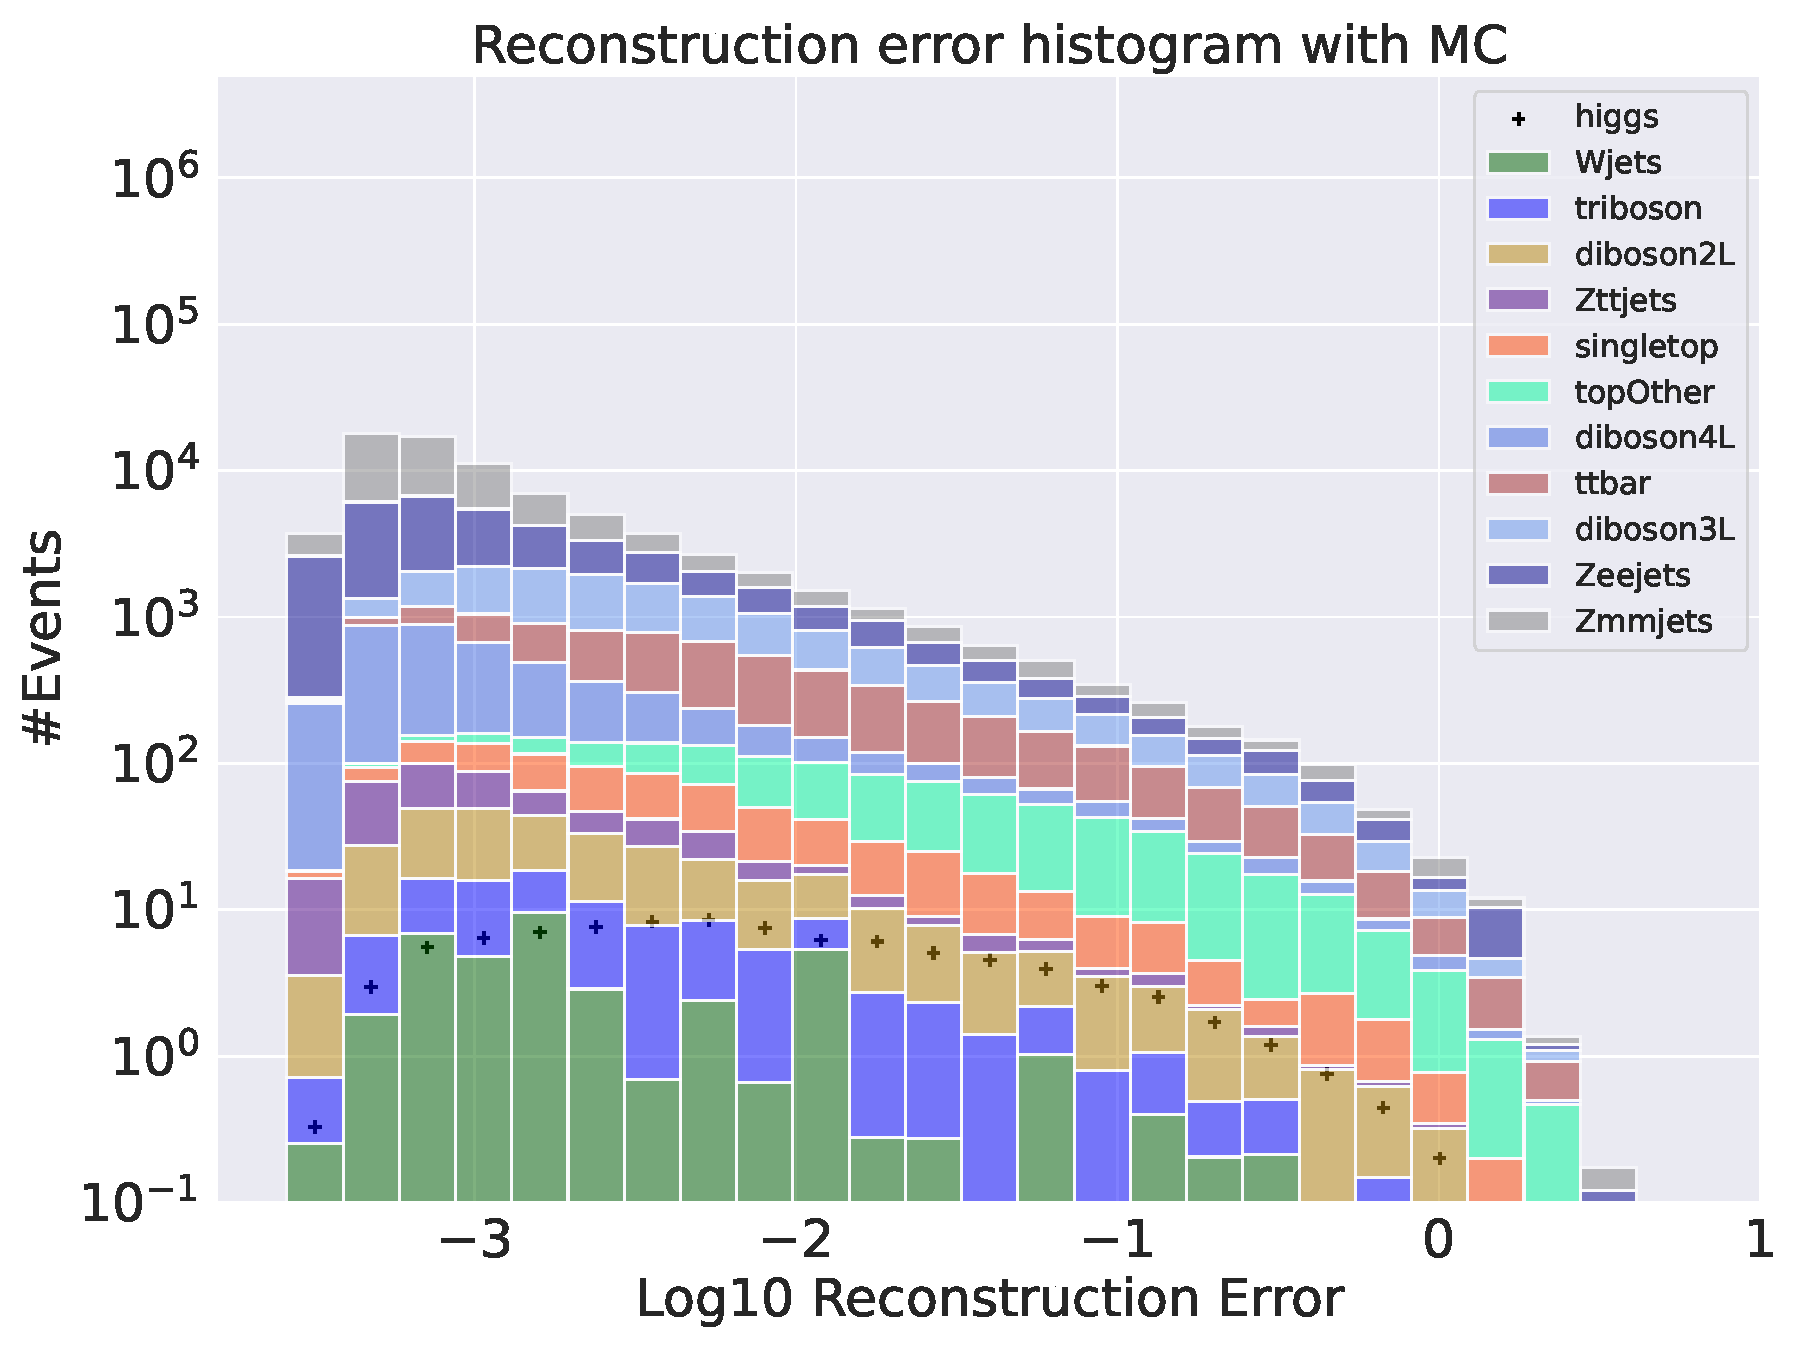
\includegraphics[width=\textwidth]{Figures/AE_testing/big/b_data_recon_big_rm3_feats_sig_higgs.pdf}
        \caption{}
        \label{fig:ae_big_higgs}
    \end{subfigure}
    \hfill        
    \caption{ }
    \label{fig:ae_big_channel2}
\end{figure}

\begin{figure}[h!]
    \centering
    \begin{subfigure}{.8\textwidth}
        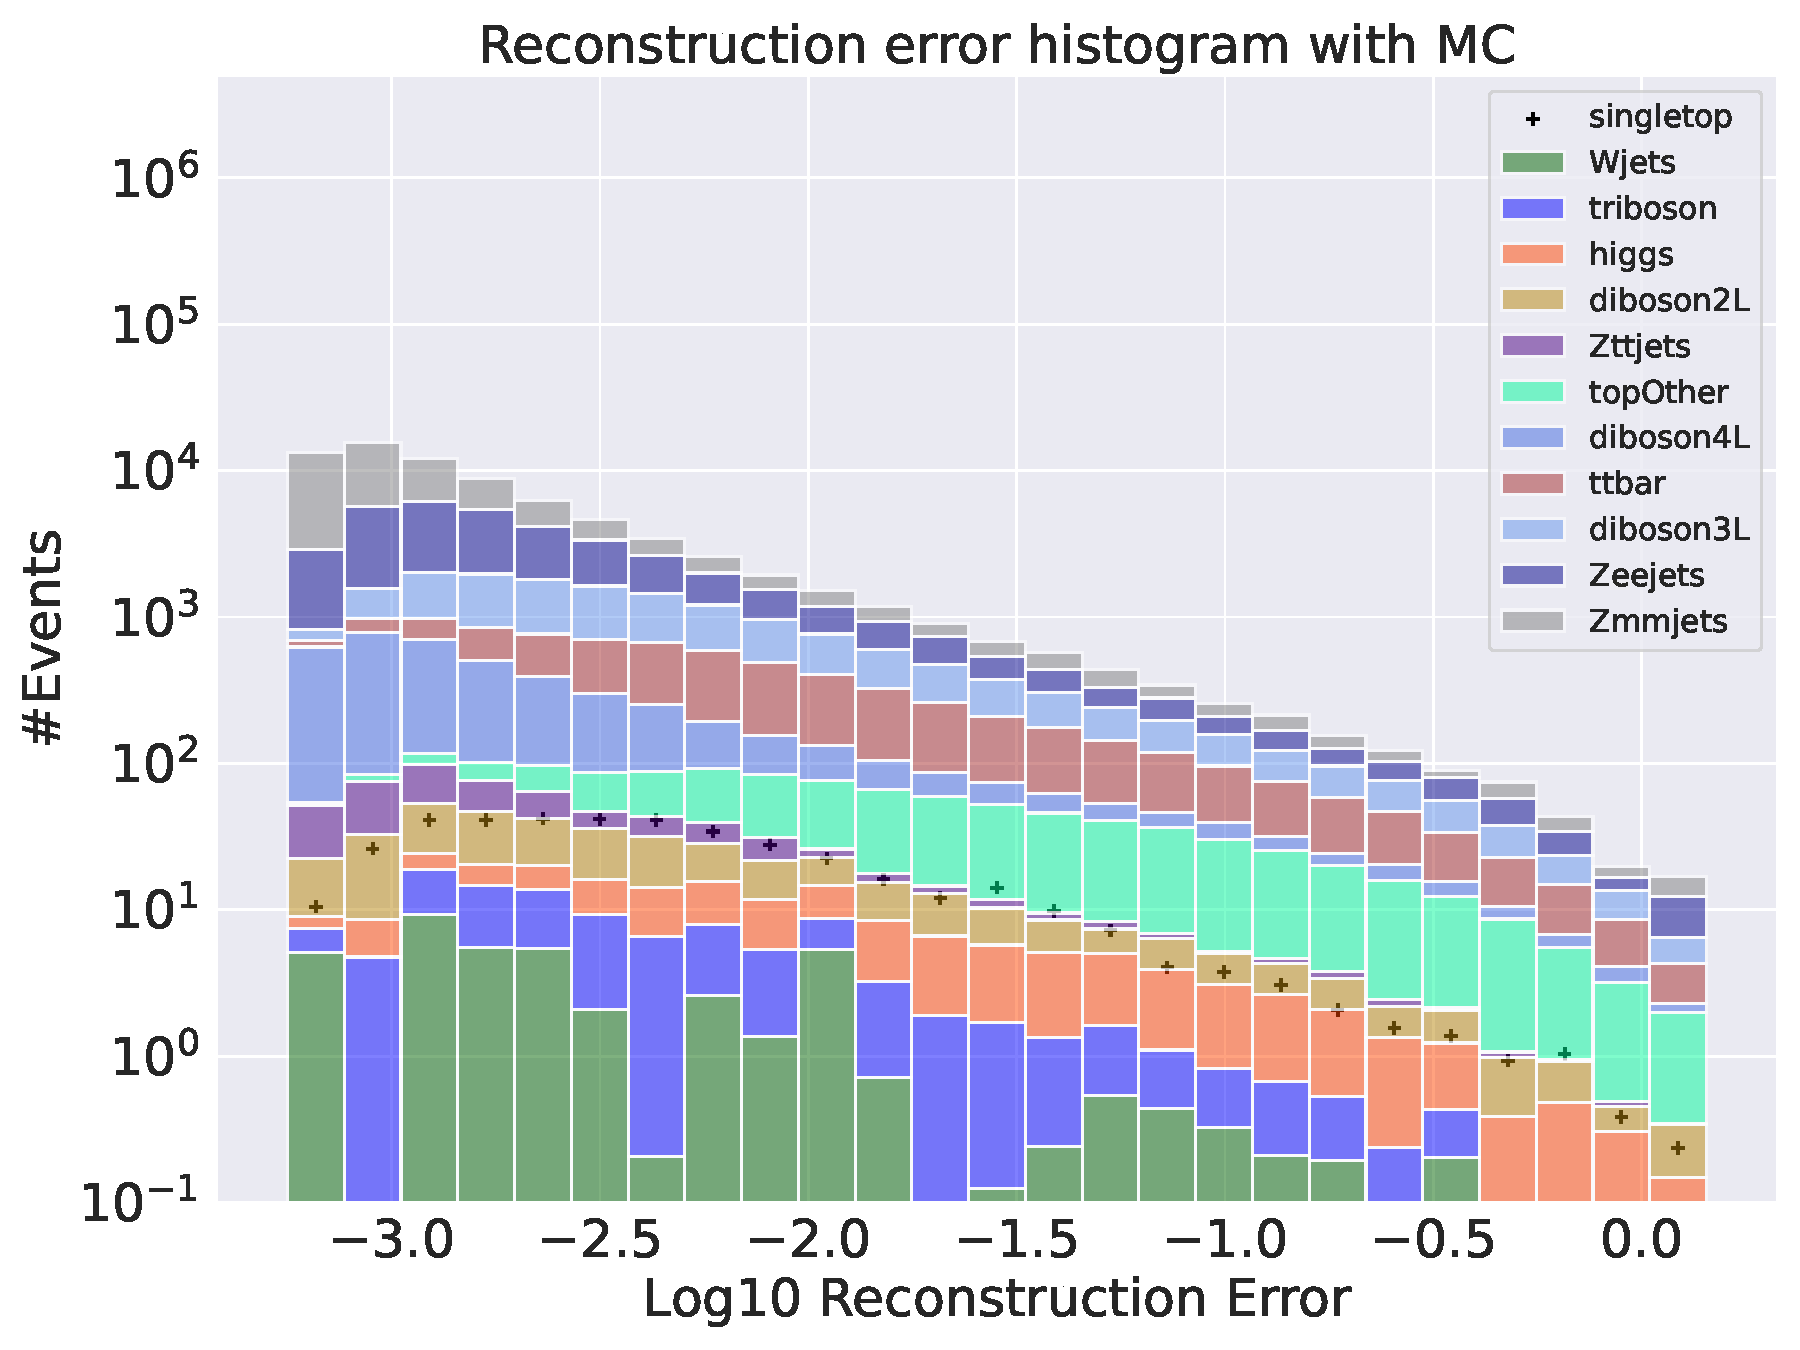
\includegraphics[width=\textwidth]{Figures/AE_testing/big/b_data_recon_big_rm3_feats_sig_singletop.pdf}
        \caption{Reconstruction error on validation SM MC from the Autoencoder. }
        \label{fig:ae_big_singletop}
    \end{subfigure}
    \hfill
    \begin{subfigure}{.8\textwidth}
        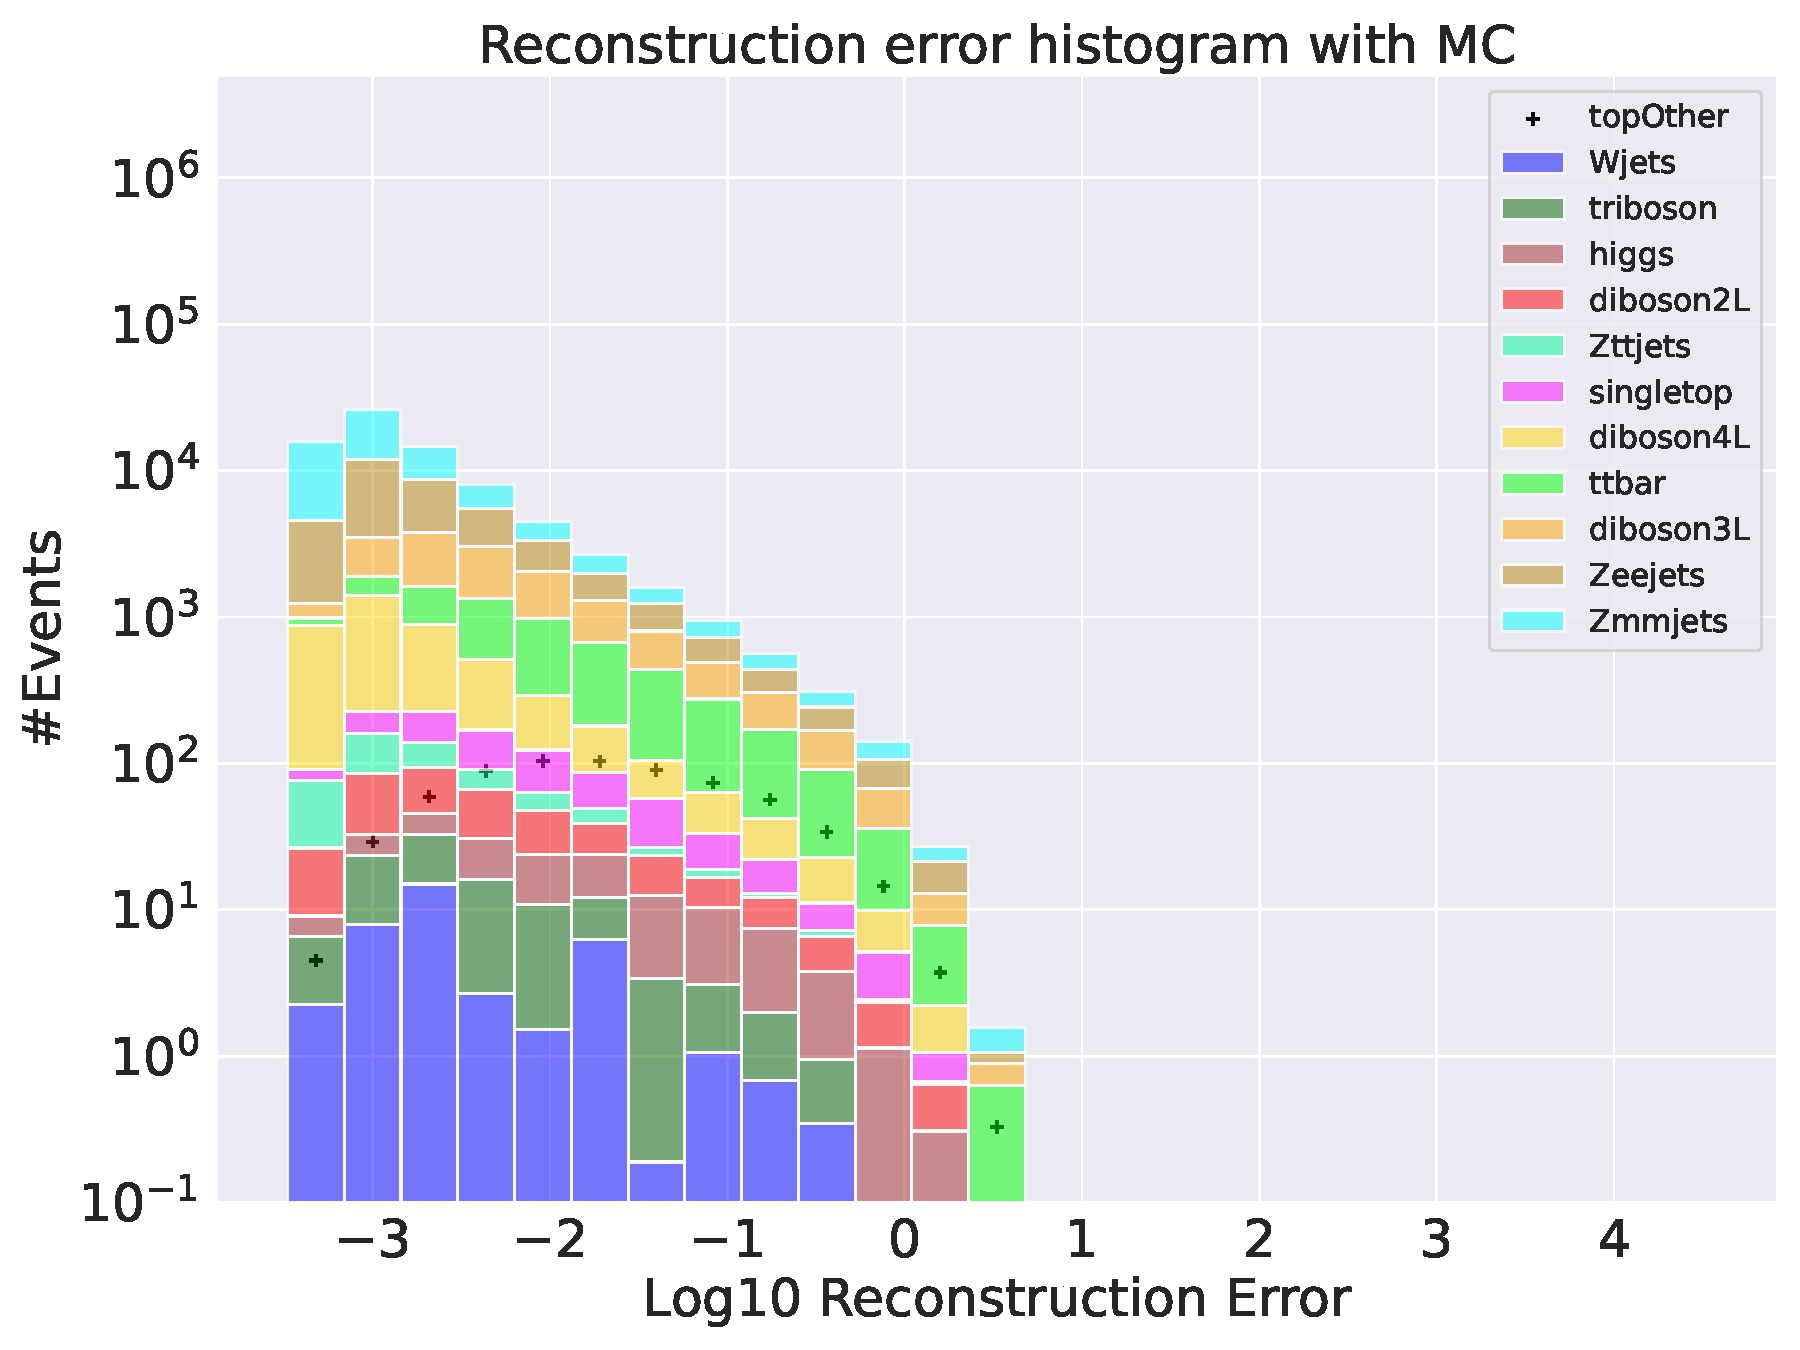
\includegraphics[width=\textwidth]{Figures/AE_testing/big/b_data_recon_big_rm3_feats_sig_topOther.pdf}
        \caption{}
        \label{fig:ae_big_topOther}
    \end{subfigure}
    \hfill        
    \caption{ }
    \label{fig:ae_big_channel3}
\end{figure}


\begin{figure}[h!]
    \centering
    \begin{subfigure}{.8\textwidth}
        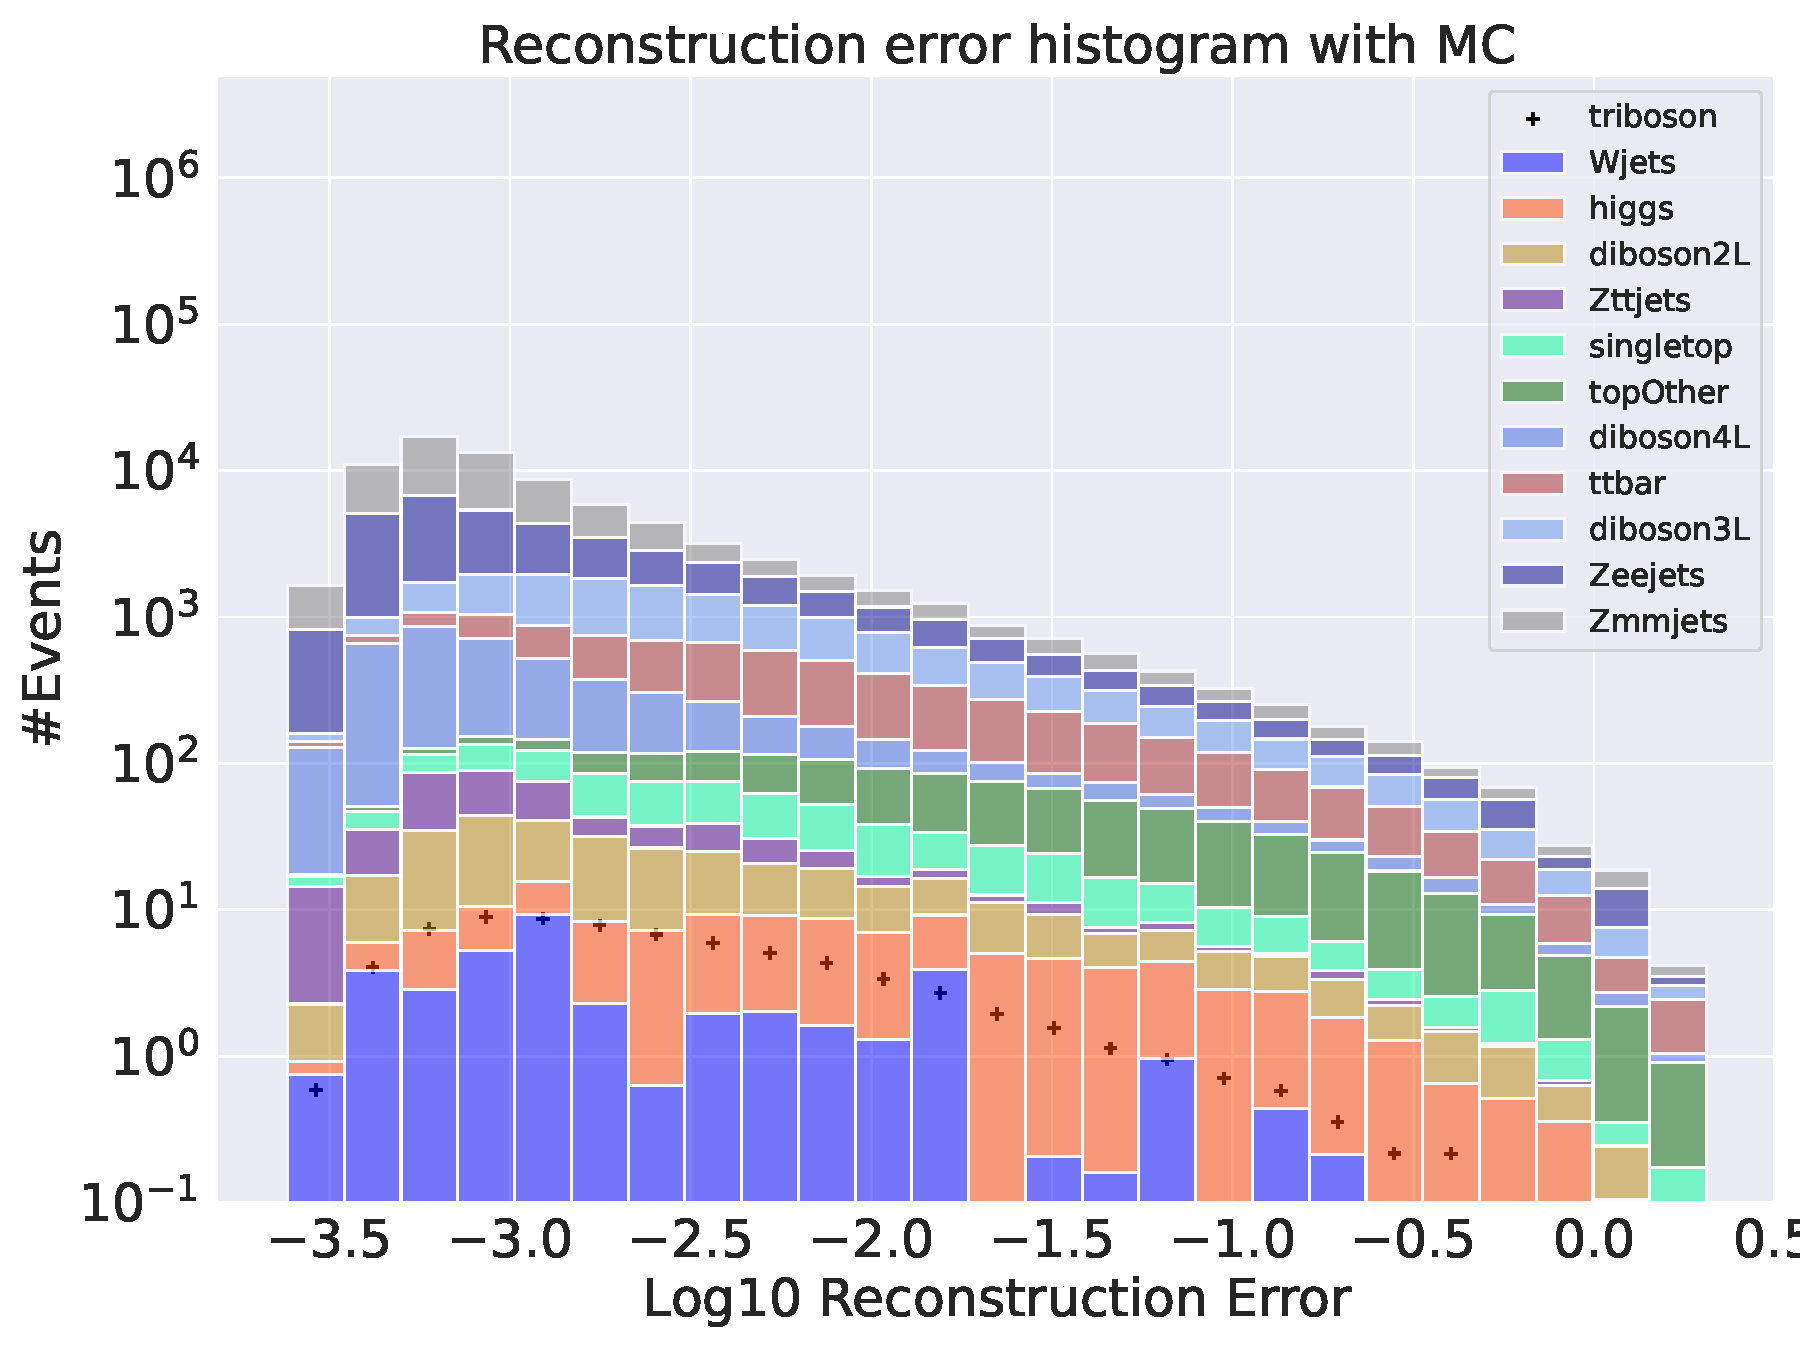
\includegraphics[width=\textwidth]{Figures/AE_testing/big/b_data_recon_big_rm3_feats_sig_triboson.pdf}
        \caption{Reconstruction error on validation SM MC from the Autoencoder. }
        \label{fig:ae_big_triboson}
    \end{subfigure}
    \hfill
    \begin{subfigure}{.8\textwidth}
        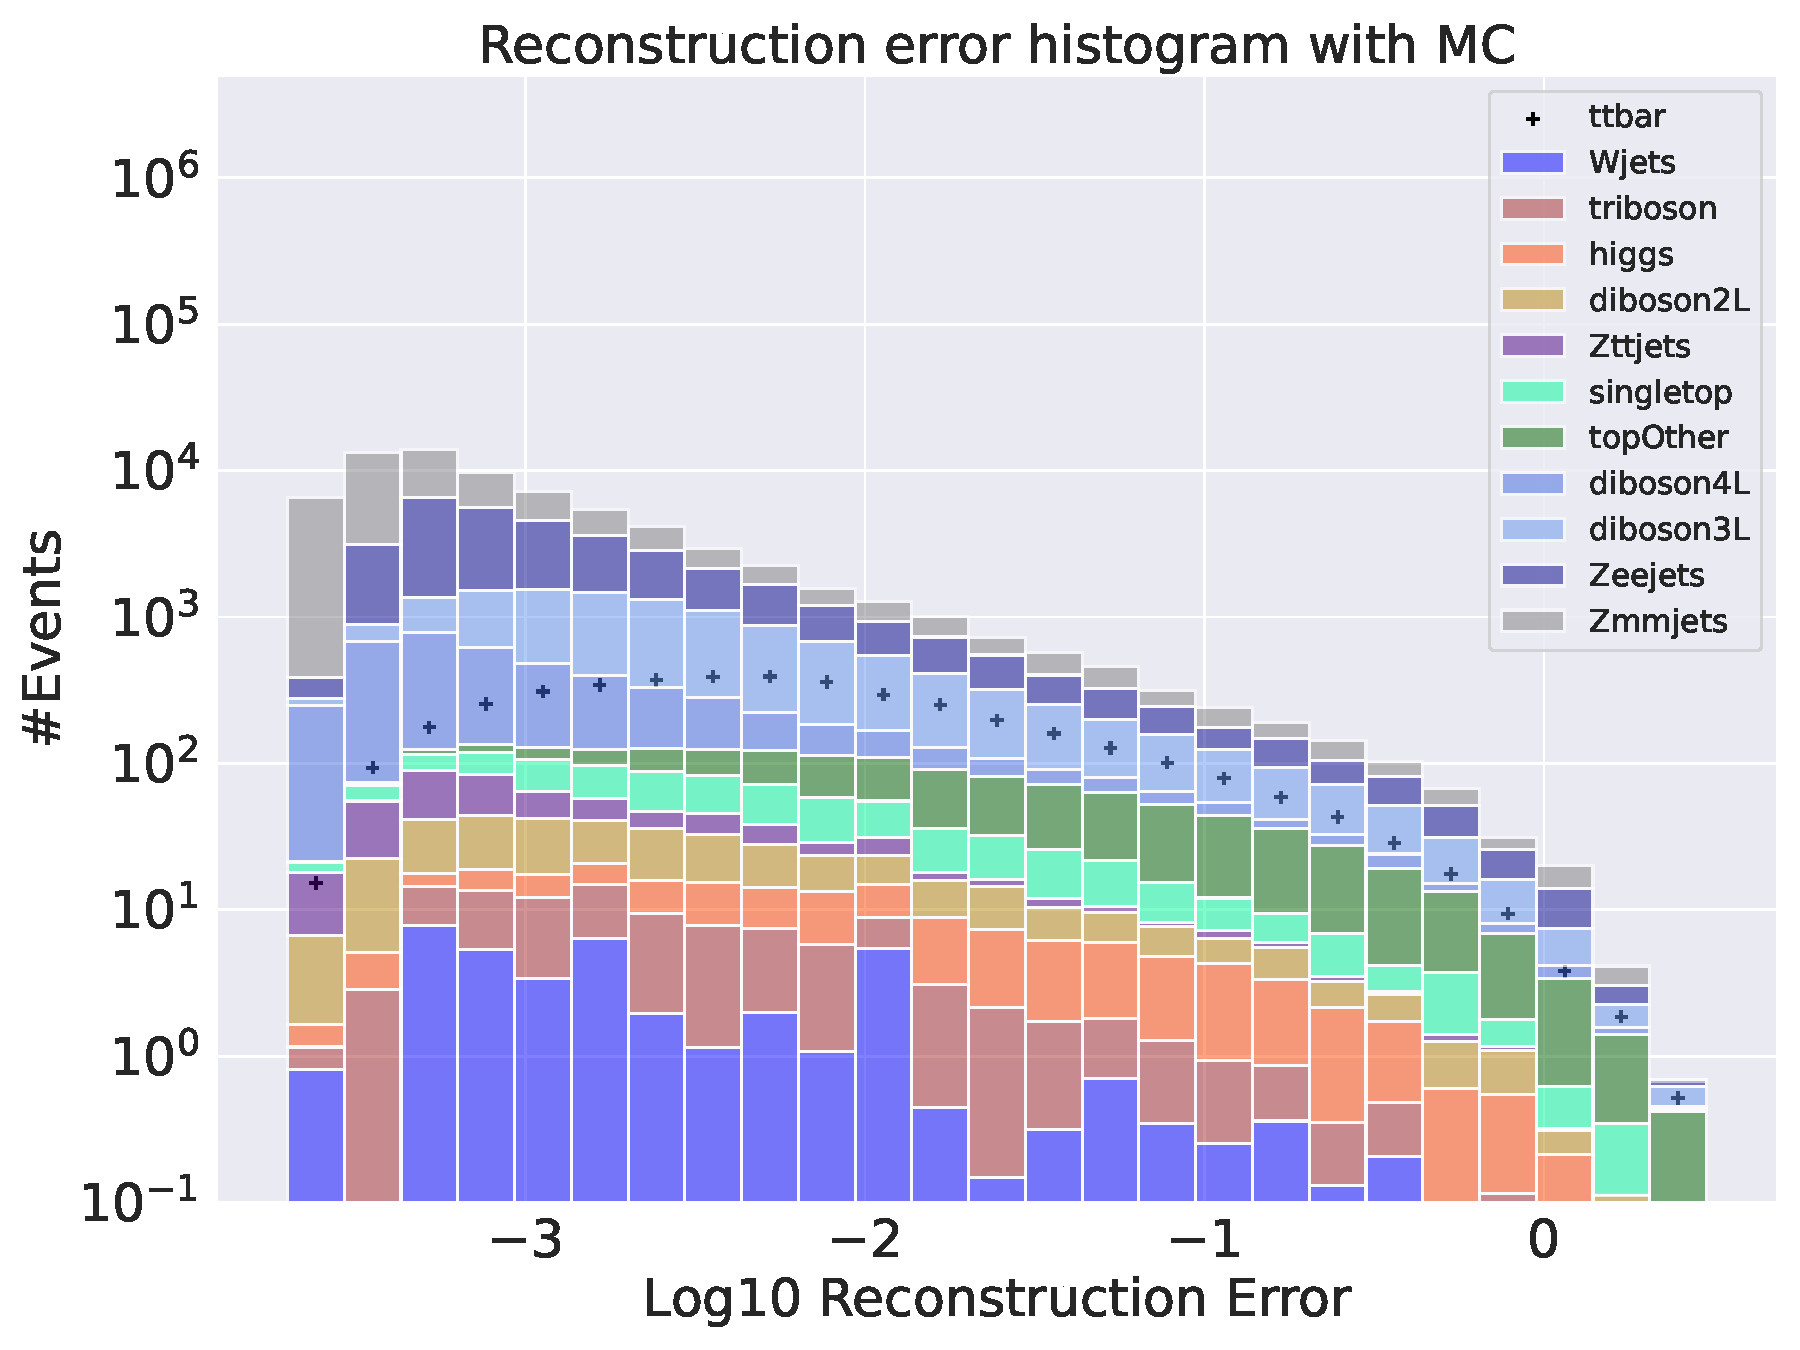
\includegraphics[width=\textwidth]{Figures/AE_testing/big/b_data_recon_big_rm3_feats_sig_ttbar.pdf}
        \caption{}
        \label{fig:ae_big_ttbar}
    \end{subfigure}
    \hfill        
    \caption{ }
    \label{fig:ae_big_channel4}
\end{figure}

\begin{figure}[h!]
    \centering
    \begin{subfigure}{.8\textwidth}
        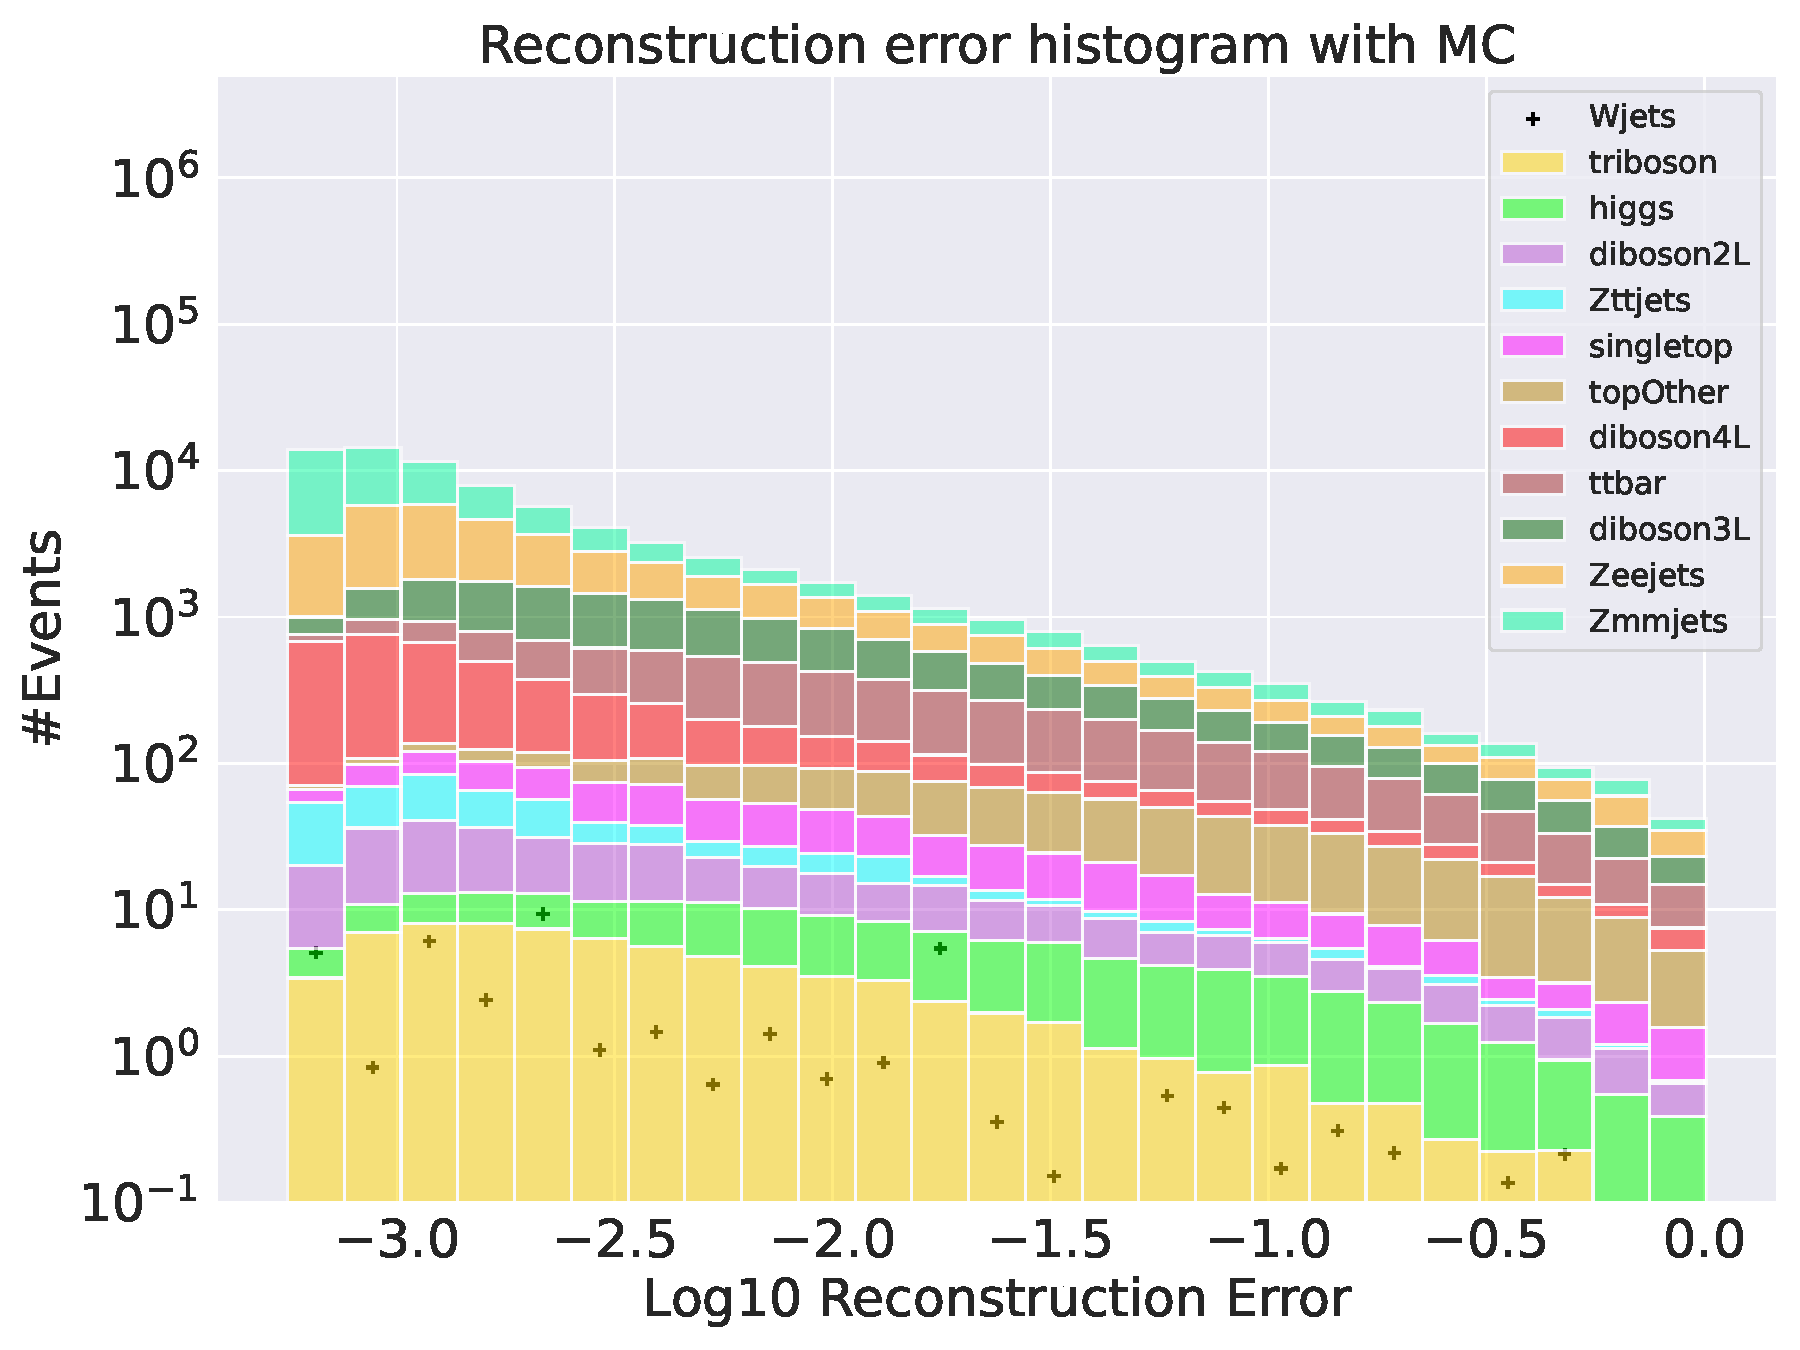
\includegraphics[width=\textwidth]{Figures/AE_testing/big/b_data_recon_big_rm3_feats_sig_Wjets.pdf}
        \caption{Reconstruction error on validation SM MC from the Autoencoder. }
        \label{fig:ae_big_wjets}
    \end{subfigure}
    \hfill
    \begin{subfigure}{.8\textwidth}
        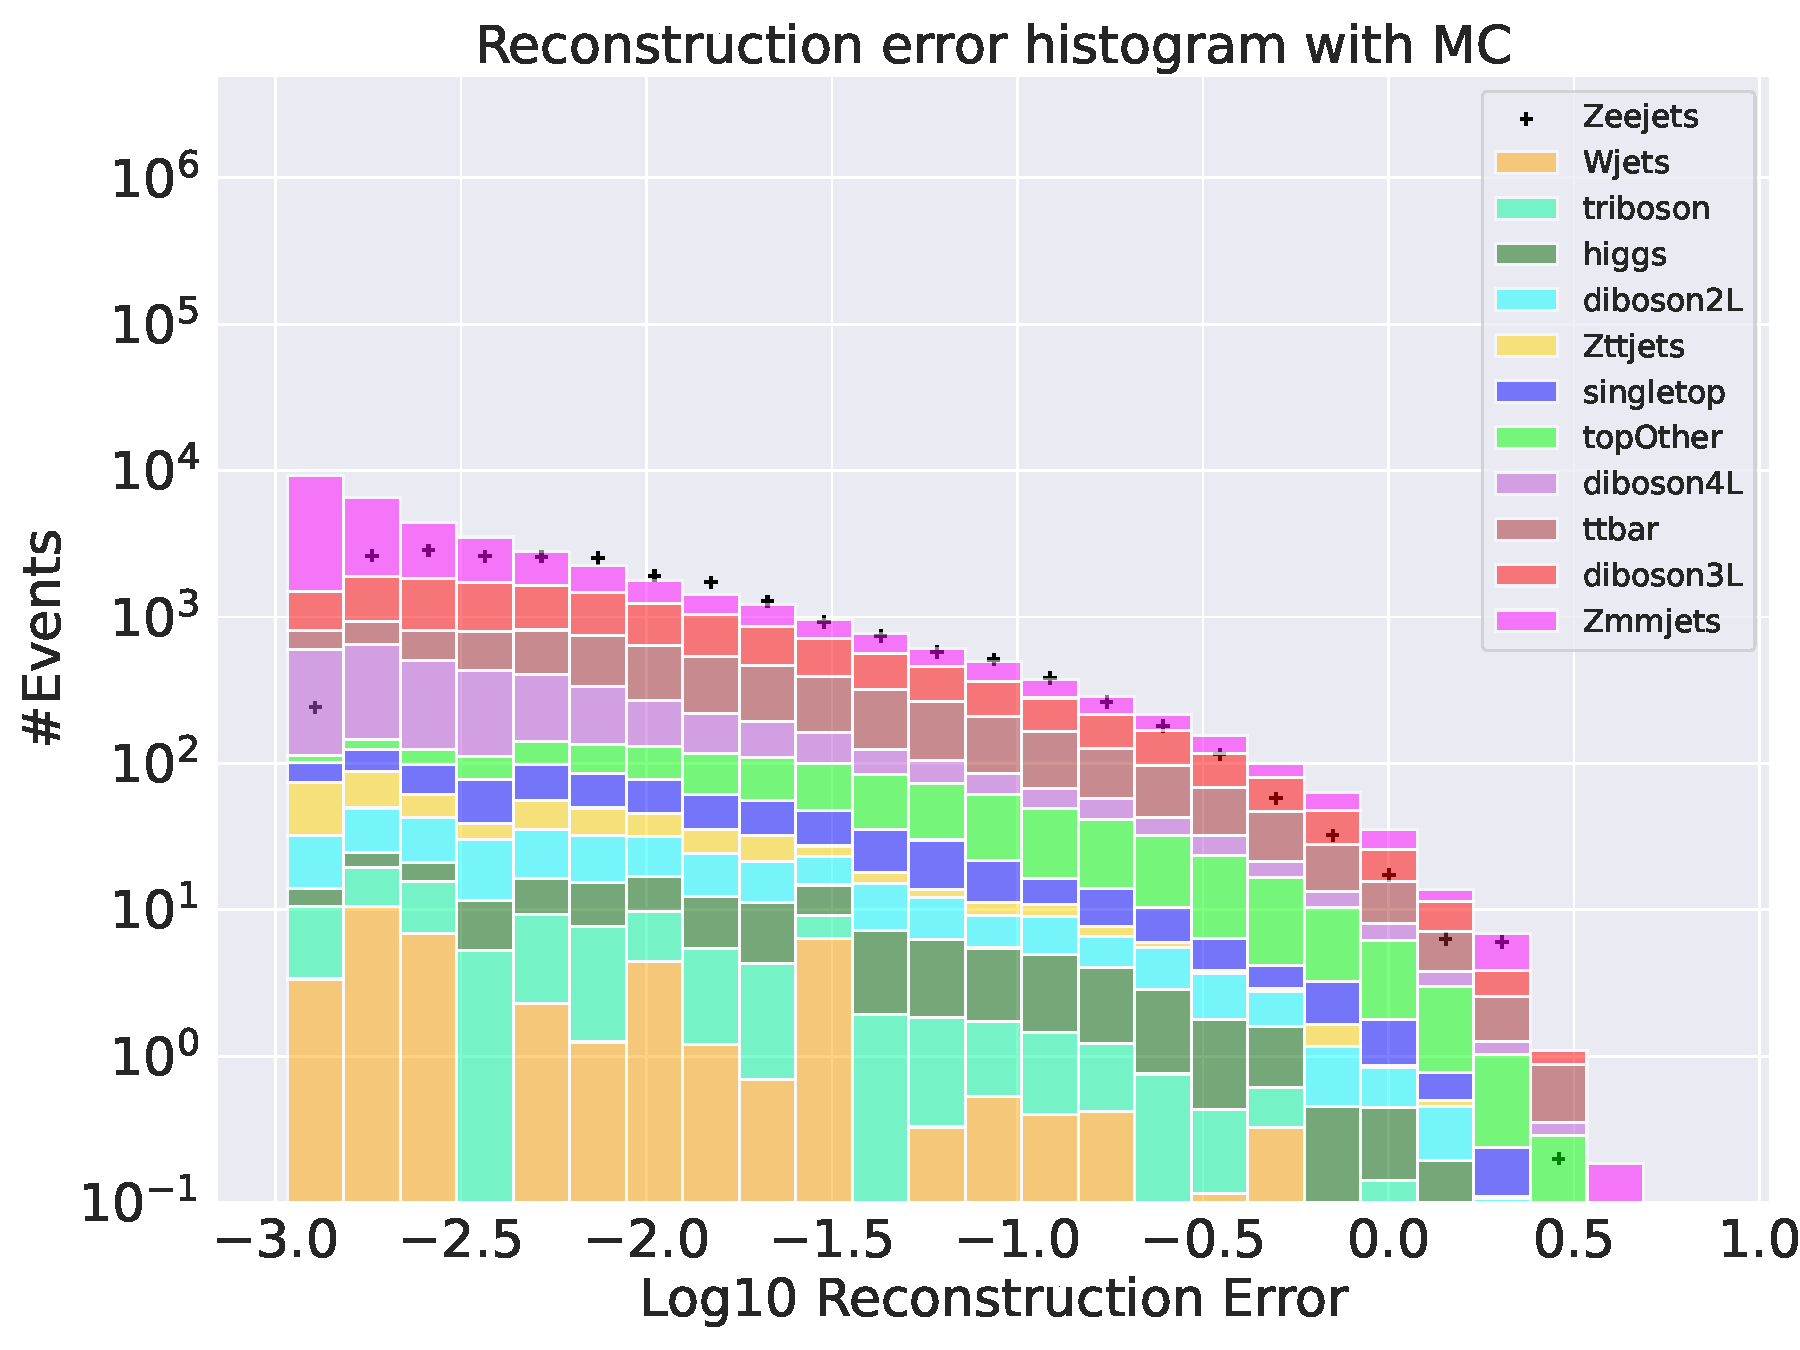
\includegraphics[width=\textwidth]{Figures/AE_testing/big/b_data_recon_big_rm3_feats_sig_Zeejets.pdf}
        \caption{}
        \label{fig:ae_big_zeejets}
    \end{subfigure}
    \hfill        
    \caption{ }
    \label{fig:ae_big_channel5}
\end{figure}

\begin{figure}[h!]
    \centering
    \begin{subfigure}{.8\textwidth}
        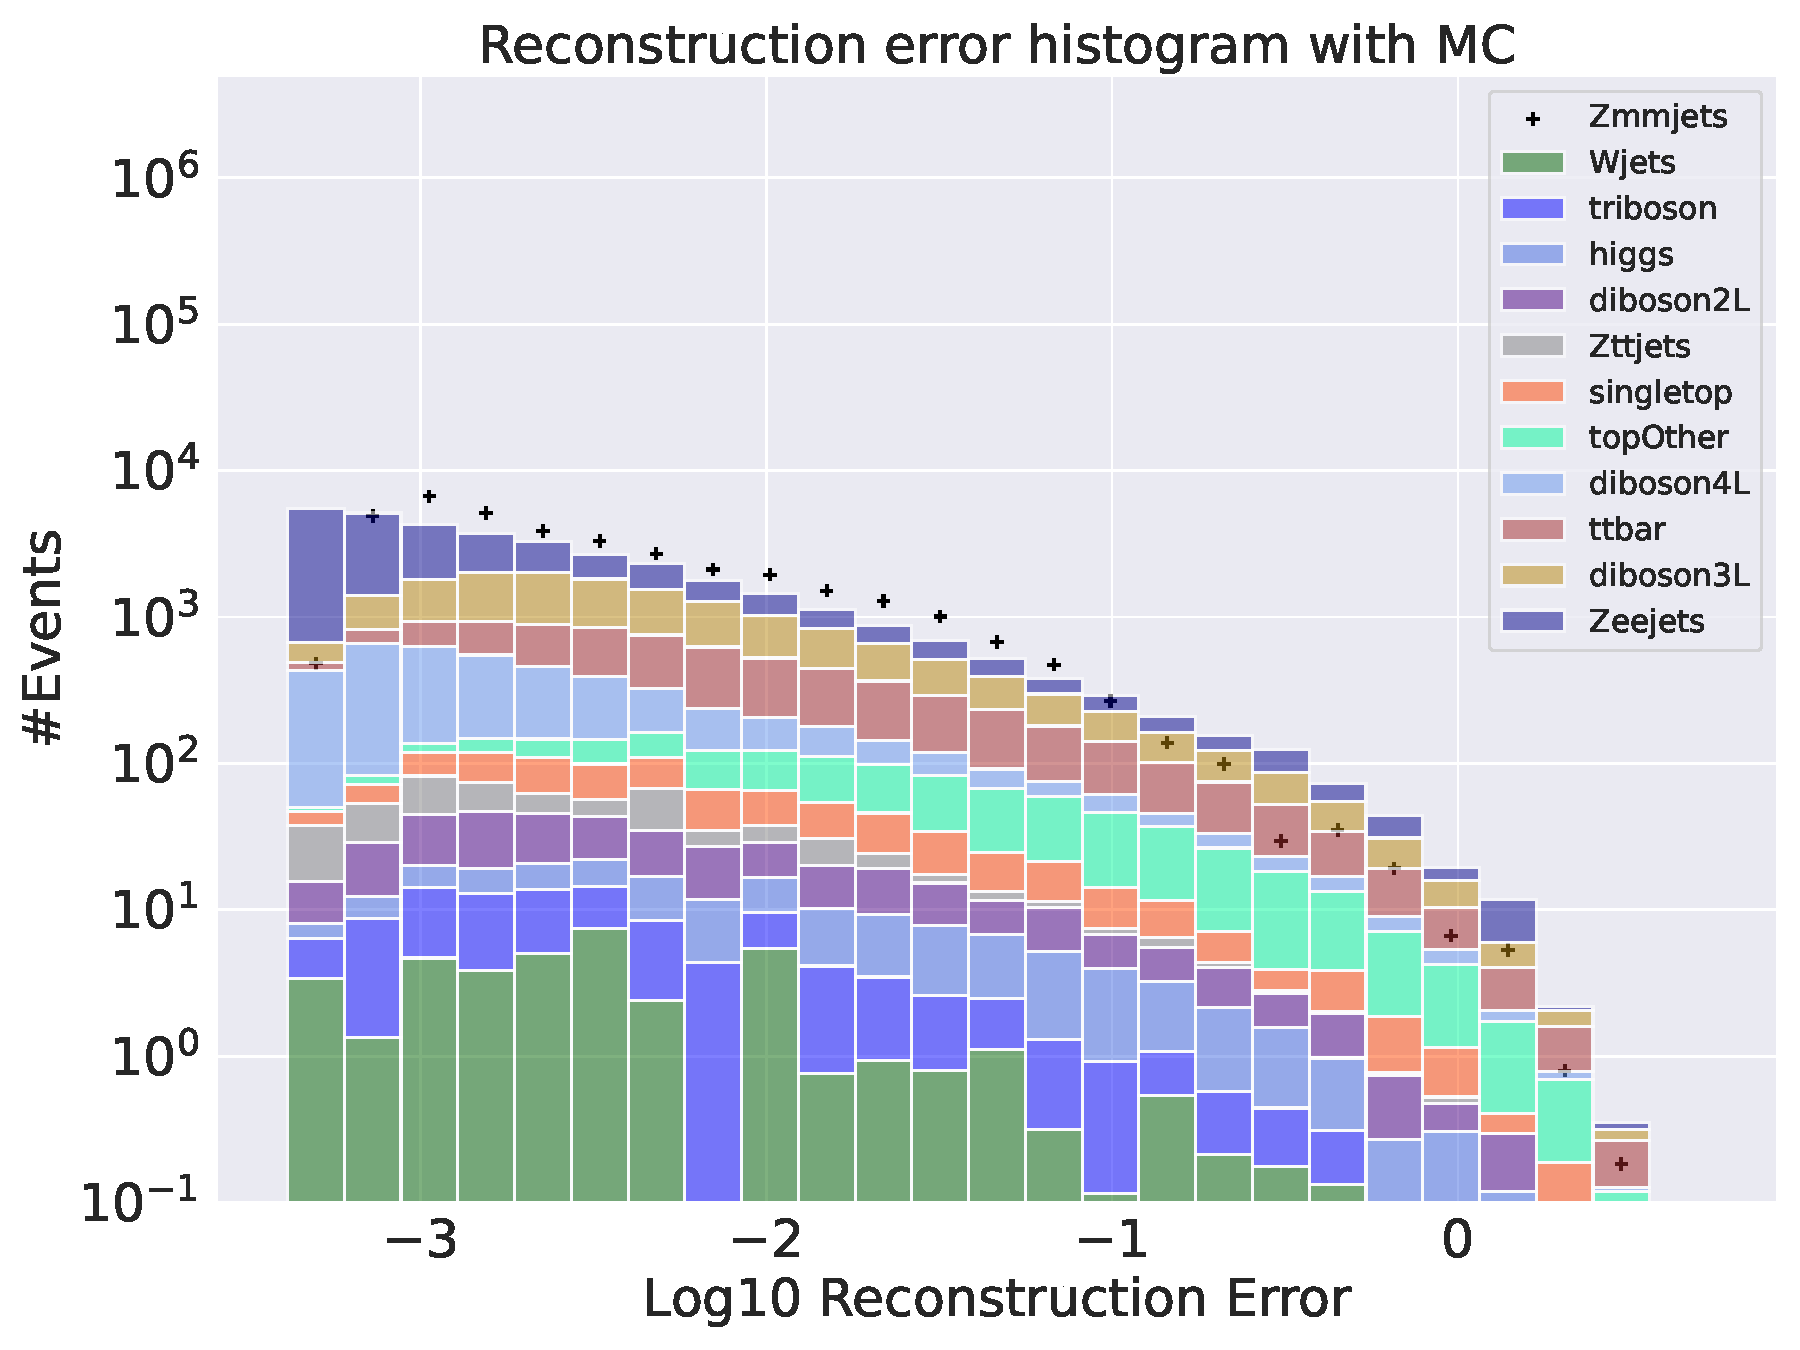
\includegraphics[width=\textwidth]{Figures/AE_testing/big/b_data_recon_big_rm3_feats_sig_Zmmjets.pdf}
        \caption{Reconstruction error on validation SM MC from the Autoencoder. }
        \label{fig:ae_big_zmmjets}
    \end{subfigure}
    \hfill
    \begin{subfigure}{.8\textwidth}
        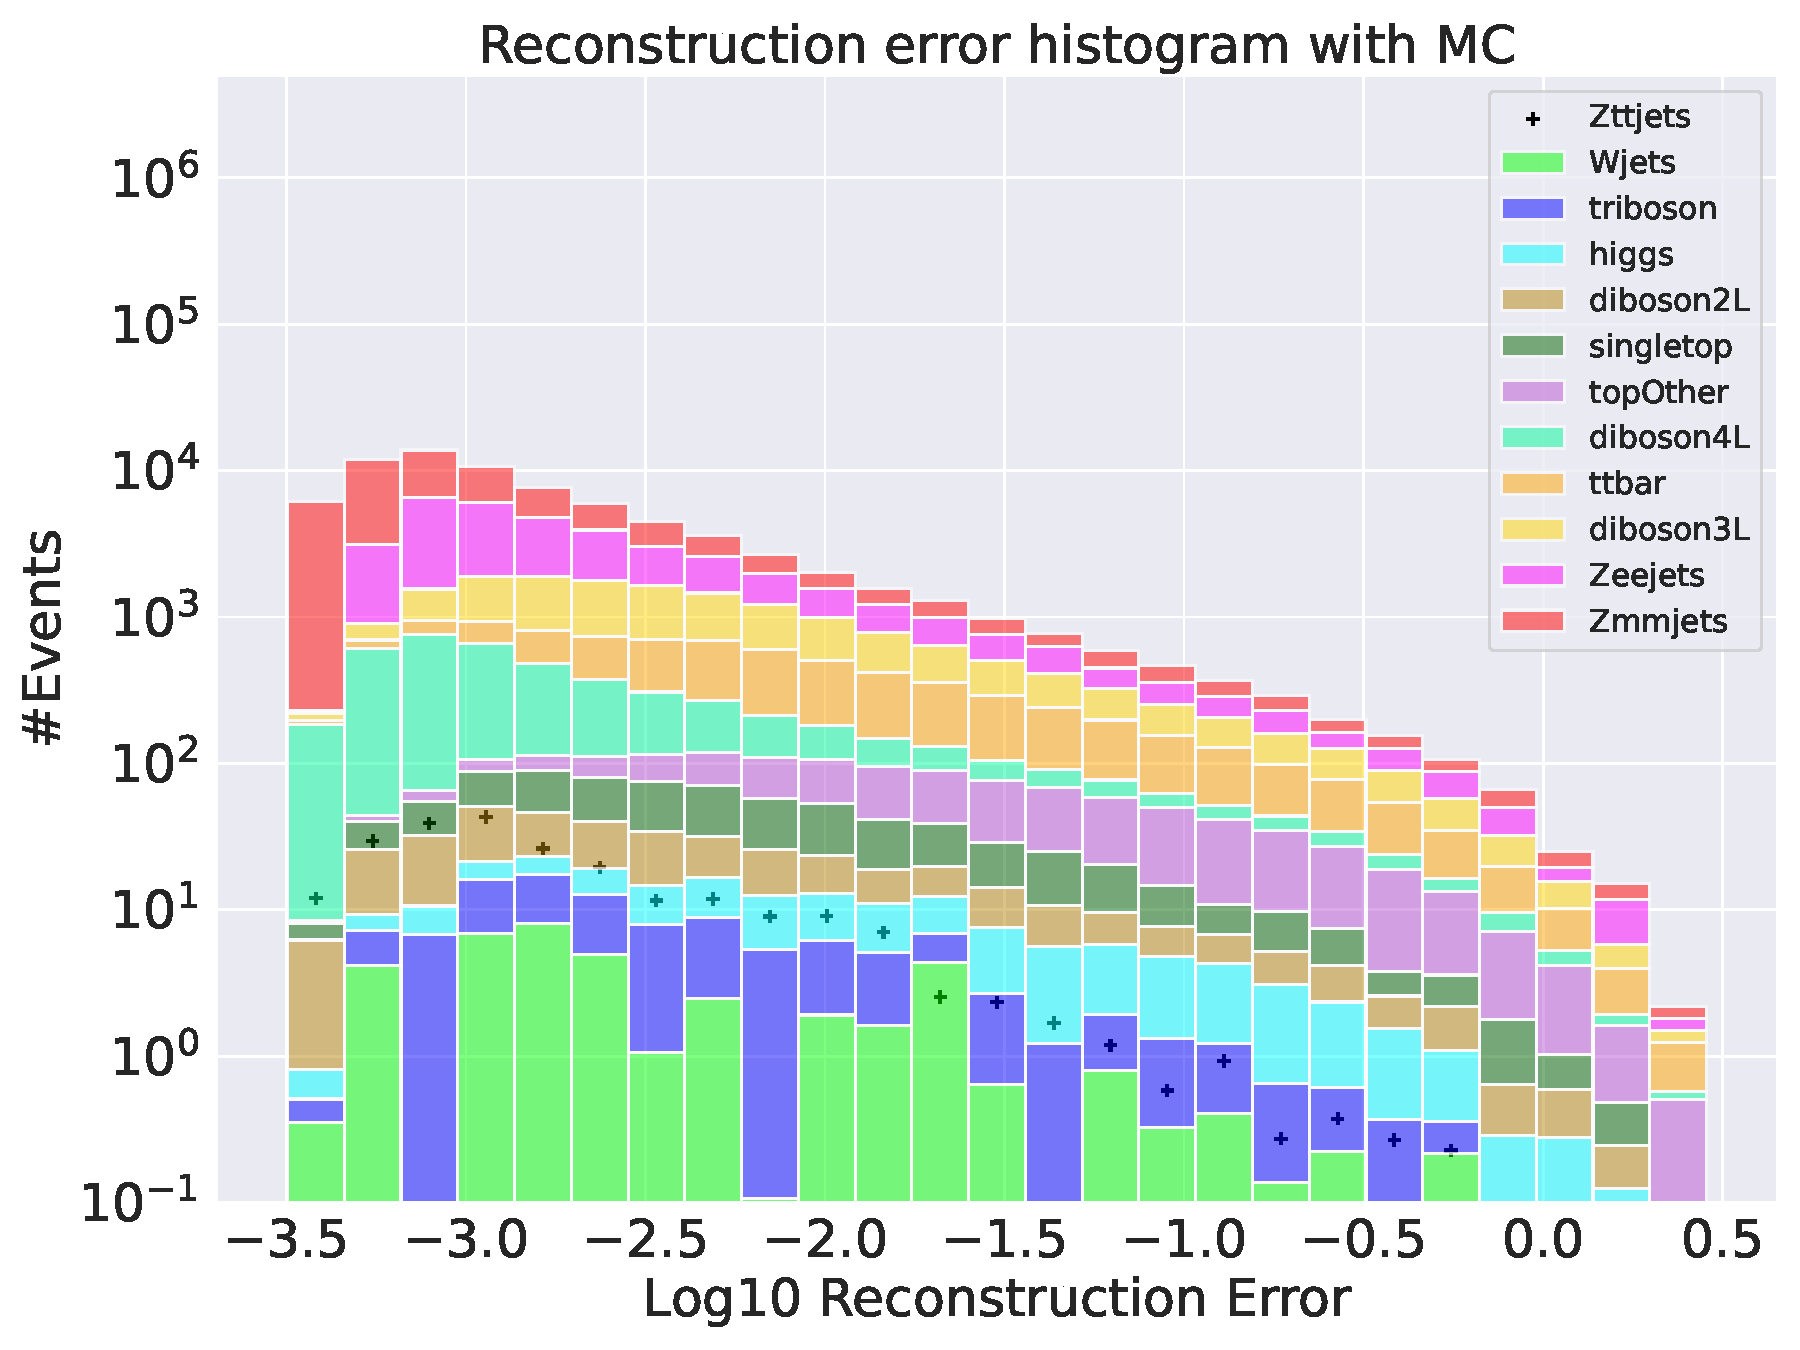
\includegraphics[width=\textwidth]{Figures/AE_testing/big/b_data_recon_big_rm3_feats_sig_Zttjets.pdf}
        \caption{}
        \label{fig:ae_big_zttjets}
    \end{subfigure}
    \hfill        
    \caption{ }
    \label{fig:ae_big_channel6}
\end{figure}